\باب{برقرار حالت بدلتی رو}
جبری تفاعل میں یکدم تبدیلی سے دور عارضی حالت اختیار کرتا ہے۔محدود قیمت کے وقتی مستقل کی صورت میں آخر کار عارضی دورانیہ گزر جاتا ہے اور دور ایک بار پھر برقرار حالت اختیار کر لیتا ہے۔جبری تفاعل میں یکدم تبدیلی کی غیر موجودگی میں دور برقرار صورت میں رہتا ہے۔اس باب میں ایسے ہی ادوار پر غور کیا جائے گا جن کے جبری تفاعل میں یکدم تبدیلی نہیں پائی جاتی۔ایسی صورت میں جبری حل ہی مکمل حل ہو گا۔اس باب میں مکمل حل  سے مراد جبری حل ہو گا۔ 
 
\حصہ{مخلوط اعداد}
\اصطلاح{حقیقی}\فرہنگ{حقیقی!عدد}\حاشیہب{real number}\فرہنگ{real!number} عدد اور \اصطلاح{خیالی}\فرہنگ{خیالی!عدد}\حاشیہب{imaginary number}\فرہنگ{imaginary!number} عدد کے مجموعے کو \اصطلاح{مخلوط}\فرہنگ{مخلوط!عدد}\حاشیہب{complex number}\فرہنگ{complex!number} عدد کہتے ہیں۔مخلوط اعداد کو \اصطلاح{مخلوط سطح}\فرہنگ{مخلوط سطح}\حاشیہب{complex plane}\فرہنگ{complex!plane} پر دکھایا جایا ہے۔مخلوط سطح پر افقی محدد حقیقی اعداد کو ظاہر کرتا ہے جبکہ عمودی محدد خیالی اعداد کو ظاہر کرتا ہے۔

شکل \حوالہ{شکل_بدلتا_مخلوط_اعداد_لکھنا}-الف میں مخلوط عدد \عددی{3+j2} دکھایا گیا ہے۔اسی شکل میں ایک مستطیل بھی دکھایا گیا ہے۔اس عدد کے حقیقی اور خیالی اجزاء مستطیل کے اطراف ہیں۔یوں مخلوط عدد کو حقیقی اور خیالی اجزاء کے مجموعے یعنی \عددی{3+j2} کے طرز پر لکھنے کو \اصطلاح{مستطیلی طرز}\فرہنگ{مستطیلی طرز}\حاشیہب{rectangular form}\فرہنگ{rectangular form} کہتے ہیں۔ 

شکل \حوالہ{شکل_بدلتا_مخلوط_اعداد_لکھنا}-الف میں مخلوط نقطہ \عددی{(3+j2)} سے محدد کے مرکز \عددی{(0,0)} تک لکیر کھینچی گئی ہے۔اس لکیر کی لمبائی \عددی{r} کو مسئلہ فیثاغورث کی مدد سے
\begin{align*}
r=\sqrt{3^2+2^2}=\sqrt{13}
\end{align*}
لکھا جا سکتا ہے۔اسی طرح افقی محدد سے لکیر تک کا زاویہ درج ذیل ہو گا۔
\begin{align*}
\theta=\tan^{-1}\frac{2}{3}=33.69^{\circ}
\end{align*}
شکل \حوالہ{شکل_بدلتا_مخلوط_اعداد_لکھنا}-ب میں اسی مخلوط عدد کو \عددی{r\phase{\theta}} کی شکل میں دکھایا گیا ہے۔مخلوط عدد کو حیطے اور زاویے سے ظاہر کرنے کو \اصطلاح{زاویائی طرز}\فرہنگ{زاویائی طرز}\حاشیہب{angular form}\فرہنگ{angular form} کہتے ہیں۔

کسی بھی مخلوط عدد \عددی{m} کو 
\begin{align}
m=x+jy\quad \quad \text{\RL{مستطیل طرز}}
\end{align}
یا
\begin{align}
m=r\phase{\theta} \quad \quad \text{\RL{زاویائی طرز}}
\end{align}
میں لکھا جا سکتا ہے جہاں مستطیلی طرز سے زاویائی طرز درج ذیل طریقے سے حاصل کی جاتی ہے
\begin{gather}
\begin{aligned}\label{مساوات_بدلتا_مستطیل_سے_زاویائی}
r&=\sqrt{x^2+y^2}\\
\theta&=\tan^{-1}\frac{y}{x}
\end{aligned}
\end{gather}
جبکہ زاویائی طرز سے مستطیل طرز درج ذیل سے حاصل کی جاتی ہے۔
\begin{gather}
\begin{aligned}
x&=r \cos \theta\\
y&=r\sin \theta
\end{aligned}
\end{gather}
%
\begin{figure}
\centering
\begin{subfigure}{0.5\textwidth}
\centering
\begin{tikzpicture}
\pgfmathsetmacro{\ang}{atan(2/3)};
\draw(0,0)--++(3.2,0)node[right]{حقیقی};
\draw(0,0)--++(0,2.7)node[left]{خیالی};
\foreach \x in {1,2,3}{\draw(\x,0)--++(0,-0.1)node[below]{$\x$};}
\foreach \y in {1,2}{\draw(0,\y)--++(-0.1,0)node[left]{$j \y$};}
\draw[gray](3,0)--++(0,2)--++(-3,0);
\draw[gray,dashed](0,0)--(3,2)node[pos=0.6,fill=white]{r};
\draw[fill](3,2) circle (1.5pt)node[right]{$3+j2$};
\draw[gray,-stealth]([shift={(0:0.8)}]0,0) arc (0:\ang:0.8);
\draw[gray](2/3*\ang:0.9)node[right]{$\theta$};
\end{tikzpicture}
\caption*{(الف) مخلوط عدد لکھنے کی مستطیل طرز۔}
\end{subfigure}%
\begin{subfigure}{0.5\textwidth}
\centering
\begin{tikzpicture}
\pgfmathsetmacro{\ang}{atan(2/3)};
\draw(0,0)--++(4.2,0)node[right]{حقیقی};
\draw(0,0)--++(0,2.7)node[left]{خیالی};
\foreach \x in {1,2,3,4}{\draw(\x,0)--++(0,-0.1)node[below]{$\x$};}
\foreach \y in {1,2}{\draw(0,\y)--++(-0.1,0)node[left]{$j \y$};}
\draw[gray](0,0)--++(3,2)node[pos=0.6,fill=white]{$\sqrt{13}$};
\draw[fill](3,2) circle (1.5pt)node[right]{$\sqrt{13}\phase{33.69^{\circ}}$};
\draw[gray,-stealth]([shift={(0:0.8)}]0,0) arc (0:\ang:0.8);
\draw[gray](2/3*\ang:0.9)node[right]{$33.69^{\circ}$};
\end{tikzpicture}
\caption*{(ب) مخلوط عدد لکھنے کی زاویائی طرز۔}
\end{subfigure}%
\caption{مخلوط اعداد کو لکھنے کے طریقے۔}
\label{شکل_بدلتا_مخلوط_اعداد_لکھنا}
\end{figure}

مخلوط اعداد کو جمع، منفی، ضرب اور تقسیم کرنے کی چند مثالیں دیکھتے ہیں۔

%================================
\ابتدا{مثال}
مخلوط اعداد \عددی{a=2+j3} اور \عددی{b=4+j5} دیے گئے ہیں۔درج ذیل حاصل کریں۔
\begin{align*}
a+b, \quad \quad a-b, \quad \quad a b, \quad \quad \frac{a}{b}
\end{align*}

حل:مخلوط اعداد جمع (منفی) کرتے وقت حقیقی اجزاء کو علیحدہ جمع (منفی) کیا جاتا ہے اور خیالی اجزاء کو علیحدہ جمع (منفی) کیا جاتا ہے۔
\begin{align*}
a+b&=(2+j3)+(4+j5)=(2+4)+j(3+5)=6+j8\\
a-b&=(2+j3)-(4+j5)=(2-4)+j(3-5)=-2-j2
\end{align*}
مخلوط اعداد کو ضرب دیتے ہوئے \عددی{j^2=(\sqrt{-1})^2=-1} لکھا جاتا ہے۔
\begin{align*}
ab&=(2+j3)(4+j5)=8+j10+j12+j^2 15=(8-15)+j(10+12)=-7+j22
\end{align*}
مخلوط اعداد کو تقسیم کرتے ہیں۔
\begin{align*}
\frac{a}{b}&=\frac{2+j3}{4+j5}\\
&=\left(\frac{2+j3}{4+j5}\right)\left(\frac{4-j5}{4-j5}\right)\\
&=\frac{8-j10+j12-j^2 15}{4^2-(j 5)^2}\\
&=\frac{23+j2}{16+25}\\
&=\frac{23}{41}+j\frac{2}{41}\\
&=0.56098+j0.04878
\end{align*}
\انتہا{مثال}
%===============================
\ابتدا{مثال}
گزشتہ مثال میں مخلوط اعداد کو زاویائی طرز پر لکھتے ہوئے \عددی{ab} اور \عددی{\tfrac{a}{b}} حاصل کریں۔

حل:مساوات \حوالہ{مساوات_بدلتا_مستطیل_سے_زاویائی} استعمال کرتے ہوئے \عددی{a=2+j3} کا حیطہ اور زاویہ حاصل کرتے ہیں۔
\begin{align*}
r_a&=\sqrt{2^2+3^2}=\sqrt{13}\\
\theta_a&=\tan^{-1}\frac{3}{2}=56.31^{\circ}
\end{align*}
یوں
\begin{align*}
a=\sqrt{13}\phase{56.31^{\circ}}
\end{align*}
لکھا جائے گا۔اسی طرح \عددی{b=4+j5} کا حیطہ اور زاویہ حاصل کرتے ہوئے
\begin{align*}
r_b&=\sqrt{4^2+5^2}=\sqrt{41}\\
\theta_b&=\tan^{-1}\frac{5}{4}=51.34^{\circ}
\end{align*}
درج ذیل لکھا جائے گا۔
\begin{align*}
b=\sqrt{41}\phase{51.34^{\circ}}
\end{align*}
اس طرح
\begin{align*}
ab&=\left(\sqrt{13}\phase{56.31^{\circ}}\right)\left(\sqrt{41}\phase{51.34^{\circ}}\right)\\
&=\sqrt{13}\sqrt{41}\phase{56.31^{\circ}+51.34^{\circ}}\\
&=\sqrt{533}\phase{107.65^{\circ}}
\end{align*}
اور
\begin{align*}
\frac{a}{b}&=\frac{\sqrt{13}\phase{56.31^{\circ}}}{\sqrt{41}\phase{51.34^{\circ}}}\\
&=\frac{\sqrt{13}}{\sqrt{41}}\phase{56.31^{\circ}-51.34^{\circ}}\\
&=\sqrt{\frac{13}{41}}\phase{4.97^{\circ}}
\end{align*}
حاصل ہوتے ہیں۔

ان جوابات کو مستطیلی طرز میں درج ذیل لکھا جائے گا جو گزشتہ مثال کے جوابات ہیں۔
\begin{align*}
ab&=\sqrt{533} \cos 107.65^{\circ}+j \sqrt{533}\sin{107.65^{\circ}}=-7+j22\\
\frac{a}{b}&=\sqrt{\frac{13}{41}} \cos 4.97^{\circ}+j\sqrt{\frac{13}{41}}\sin 4.97^{\circ}=0.56098+j0.04878
\end{align*}
\انتہا{مثال}
%======================

ہم نے دیکھا کہ زاویائی طرز میں لکھا مخلوط عدد \عددی{a=r\phase{\theta}}  مستطیل طرز میں بھی لکھا جا سکتا ہے یعنی
\begin{align}
a=r\phase{\theta}=r \cos \theta +j r \sin \theta
\end{align}
\اصطلاح{یولر مساوات}\فرہنگ{یولر مساوات}\حاشیہب{Euler's equation}\فرہنگ{Euler's equation} درج ذیل ہے۔
\begin{align}
e^{j \theta}=\cos \theta+j \sin \theta
\end{align}
مندرجہ بالا دو مساوات کو ملاتے ہوئے درج ذیل لکھا جا سکتا ہے۔
\begin{align}\label{مساوات_بدلتا_مخلوط_عدد_طرز_لکھائی}
r\phase{\theta}=r e^{j\theta}=r\left(\cos \theta+j  \sin \theta\right)
\end{align}
%=================================
\ابتدا{مثال}
مخلوط عدد \عددی{m=5-j12} کو زاویائی طرز میں لکھیں۔

حل:مساوات \حوالہ{مساوات_بدلتا_مستطیل_سے_زاویائی} کے استعمال سے درج ذیل حاصل کرتے ہیں
\begin{align*}
r&=\sqrt{5^2+12^2}=13\\
\theta&=\tan^{-1}\frac{-12}{5}=-67.38^{\circ}
\end{align*}
لہٰذا درج ذیل لکھے جا سکتے ہیں۔
\begin{align*}
m&=13 e^{-j67.38^{\circ}}\\
m&=13\phase{-67.38^{\circ}}
\end{align*}
\انتہا{مثال}
%======================
\حصہ{سائن نما تفاعل}
\اصطلاح{سائن نما}\فرہنگ{سائن نما}\حاشیہب{sinusoidal}\فرہنگ{sinusoidal} تفاعل سے مراد \اصطلاح{سائن} تفاعل \عددی{\sin \theta} اور \اصطلاح{کوسائن} تفاعل \عددی{\cos \theta} ہیں۔شکل \حوالہ{شکل_بدلتی_رو_سائن_تفاعل}-الف میں رداس \عددی{A_0} کے گول دائرے پر ایک نقطہ یکساں رفتار کے ساتھ، گھڑی کی گردش کی الٹ سمت میں، حرکت کر رہا ہے۔یہ دائرہ \اصطلاح{کارتیسی محدد}\فرہنگ{کارتیسی محدد}\حاشیہب{Cartesian coordinates}\فرہنگ{Cartesian coordinates} کے مرکز \عددی{(0,0)} پر پایا جاتا ہے۔لمحہ \عددی{t} پر زاویہ \عددی{\phase{aox}} کی قیمت \عددی{\theta} کے برابر ہے۔نقطے سے \عددی{x} محدد پر عمودی لکیر محدد کو  \عددی{x(t)}  پر ٹکراتی ہے جبکہ \عددی{y} محدد پر عمودی لکیر \عددی{y(t)} پر ٹکراتی ہے۔شکل کو دیکھتے ہوئے درج ذیل لکھا جا سکتا ہے
\begin{align}\label{مساوات_بدلتا_سائن_نما_تفاعل_الف}
y(t)&=A_0 \sin \theta
\end{align}
جہاں \عددی{A_0} موج کی چوٹی ہے جسے موج کا \اصطلاح{حیطہ}\فرہنگ{حیطہ}\حاشیہب{amplitude}\فرہنگ{amplitude} کہتے ہیں اور \عددی{\theta} کو تفاعل کا \اصطلاح{دلیل}\فرہنگ{دلیل}\حاشیہد{ایک ماہر ریاضی اپنی خیالی دنیا میں کوسائن \عددی{\cos \theta} تفاعل کے ساتھ بحث میں مصورف ہوتا ہے۔ماہر ریاضی تفاعل کو دلیل کے طور پر صفر پیش کرتا ہے۔تفاعل اس کا فوراً جواب اکائی \عددی{(\cos 0=1)} دیتا ہے۔}\حاشیہب{argument}\فرہنگ{argument} کہتے ہیں۔اس مساوات میں \عددی{\theta} از خود وقت\عددی{t} پر منحصر ہے۔

 گردش کرتا نقطہ ایک چکر میں \عددی{360^{\circ}} درجے کا زاویہ یعنی \عددی{2\pi} ریڈیئن طے کرتا ہے۔ایک چکر کاٹنے کے لئے درکار دورانیے کو \اصطلاح{دوری عرصہ}\فرہنگ{دوری عرصہ}\حاشیہب{time period}\فرہنگ{time period} کہتے ہیں جسے \عددی{T} سے ظاہر کیا جاتا ہے۔
%=========================
\ابتدا{مشق}
شکل \حوالہ{شکل_بدلتی_رو_سائن_تفاعل}-الف میں نقطہ ایک چکر \عددی{\SI{20}{\milli\second}} میں پورا کرتا ہے۔یہ نقطہ ایک سیکنڈ میں کتنے چکر پورا کرے گا۔یہ نقطہ ایک سیکنڈ میں کتنے ریڈیئن کا زاویہ طے کرتا ہے۔

جوابات:\عددی{50} چکر، \عددی{100\pi \, \si{\radian}}
\انتہا{مشق}
%========================

اگر ایک چکر کاٹنے کے لئے \عددی{T} سیکنڈ کا وقت درکار ہو تب ایک سیکنڈ میں چکروں کی تعداد  \عددی{\tfrac{1}{T}} ہو گی جسے \اصطلاح{تعدد}\فرہنگ{تعدد}\حاشیہب{frequency}\فرہنگ{frequency} کہتے اور \عددی{f} سے ظاہر کرتے ہیں۔
\begin{align}
f=\frac{1}{T}
\end{align}
تعدد کی اکائی \اصطلاح{ہرٹز}\فرہنگ{ہرٹز}\حاشیہب{Hertz}\فرہنگ{Hertz} ہے جسے \عددی{\si{\hertz}} سے ظاہر کیا جاتا ہے۔

ایک چکر \عددی{2\pi} ریڈیئن کو کہتے ہیں لہٰذا \عددی{f} چکر سے مراد \عددی{2\pi f} ریڈیئن کا زاویہ ہے۔یوں \عددی{f} تعدد پر گردش کرتا نقطہ ایک سیکنڈ میں \عددی{2\pi f} ریڈیئن کا زاویہ طے کرے گا یعنی اس کی \اصطلاح{زاویائی رفتار}\فرہنگ{زاویائی رفتار}\حاشیہب{angular speed}\فرہنگ{angular speed} کی قیمت \عددی{2\pi f} ہو گی۔زاویائی رفتار کو \عددی{\omega} سے ظاہر کیا جاتا ہے جبکہ اس کی اکائی ریڈیئن فی سیکنڈ \عددی{\si{\radian\per\second}} ہے۔
\begin{align}
\omega=2\pi f
\end{align}
زاویائی رفتار \عددی{\omega} سے گردش کرتا ہوا نقطہ \عددی{t} سیکنڈ میں \عددی{2\pi f t} ریڈیئن کا زاویہ طے کرے گا۔یوں اگر \عددی{t=0} پر نقطہ عین \عددی{x} محدد کے مثبت حصے پر ہو تب لمحہ \عددی{t} پر
\begin{align}
\theta=\omega t=2\pi f t
\end{align}
لکھا جائے گا۔یوں مساوات  \حوالہ{مساوات_بدلتا_سائن_نما_تفاعل_الف} کو
\begin{gather}
\begin{aligned}\label{مساوات_بدلتا_سائن_نما_تفاعل_ب}
y(t)&=A_0 \sin 2\pi f t\\
&=A_0\sin \frac{2\pi}{T}t\\
&=A_0 \sin \omega t
\end{aligned}
\end{gather}
لکھا جا سکتا ہے۔

برقی میدان میں \عددی{y(t)} وقت کے ساتھ بدلتے دباو یا وقت کے ساتھ بدلتی رو کو ظاہر کر سکتی ہے۔مساوات \حوالہ{مساوات_بدلتا_سائن_نما_تفاعل_ب} میں دیے تفاعل، جسے شکل \حوالہ{شکل_بدلتی_رو_سائن_تفاعل}-ب میں دکھایا گیا ہے،  کا آزاد متغیرہ وقت \عددی{t} ہے۔آپ دیکھ سکتے ہیں کہ یہ تفاعل ہر \عددی{T} سیکنڈ کے بعد اپنے آپ کو دہراتا ہے۔ اس حقیقت کو ریاضی میں درج ذیل لکھا جاتا ہے۔
\begin{align}
y(t+T)=y( t)
\end{align}
جس سے مراد یہ ہے کہ تفاعل کی قیمت لمحہ \عددی{t} اور لمحہ \عددی{t+T} پر برابر ہیں۔

\begin{figure}
\centering
\begin{subfigure}{0.5\textwidth}
\centering
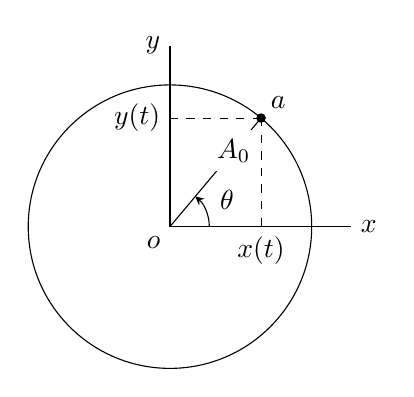
\begin{tikzpicture}
\pgfmathsetmacro{\ang}{50}
\pgfmathsetmacro{\rad}{1.8}
\pgfmathsetmacro{\xp}{\rad*cos(\ang)}
\pgfmathsetmacro{\yp}{\rad*sin(\ang)}
\draw[](0,0)--++(\rad+0.5,0)node[right]{$x$};
\draw[](0,0)--++(0,\rad+0.5)node[left]{$y$};
\draw[](0,0) circle (\rad);
\draw[fill](\ang:\rad) circle (1.5pt);
\draw(0,0)node[below left]{$o$}--++(\ang:\rad)node[pos=0.7,fill=white]{$A_0$}node[above right]{$a$};
\draw[-stealth] ([shift={(0:0.5)}]0,0) arc (0:\ang:0.5);
\draw(\ang/2:0.8)node{$\theta$};
\draw[dashed](\xp,\yp)--(\xp,0)node[below]{$x(t)$};
\draw[dashed](\xp,\yp)--(0,\yp)node[left]{$y(t)$};
\end{tikzpicture}
\caption*{الف}
\end{subfigure}
\begin{subfigure}{0.5\textwidth}
\centering
\begin{tikzpicture}
\begin{axis}[kStyleCircuitsA,small, xlabel=$t$, ylabel=$y(t)$, xtick={90,180,270,360},xticklabels={$\dfrac{T}{4}$,$\dfrac{T}{2}$,$\dfrac{3T}{2}$,$T$},ytick={-1,1},yticklabels={$-A_0$,$A_0$},
]
\addplot[domain=0:400,samples=100]{sin(x)};
\draw[gray,dashed](axis cs:0,1)--(axis cs:90,1);
\draw[gray,dashed](axis cs:0,-1)--(axis cs:270,-1);
\end{axis}%
\end{tikzpicture}%
\caption*{(ب)}
\end{subfigure}%
\begin{subfigure}{0.5\textwidth}
\centering
\begin{tikzpicture}
\begin{axis}[kStyleCircuitsA,small, xlabel=$\omega t$, ylabel=$y(\omega t)$, xtick={90,180,270,360},xticklabels={$\dfrac{\pi}{2}$,$\pi$,$\dfrac{3\pi}{2}$,$2\pi$},ytick={-1,1},yticklabels={$-A_0$,$A_0$},
]
\addplot[domain=0:400,samples=100]{sin(x)};
\draw[gray,dashed](axis cs:0,1)--(axis cs:90,1);
\draw[gray,dashed](axis cs:0,-1)--(axis cs:270,-1);
\end{axis}%
\end{tikzpicture}%
\caption*{(پ)}
\end{subfigure}%
\caption{سائن موج۔}
\label{شکل_بدلتی_رو_سائن_تفاعل}
\end{figure}%

مساوات \حوالہ{مساوات_بدلتا_سائن_نما_تفاعل_ب} کے خط کو \عددی{\omega t} کے ساتھ بھی کھینچا جا سکتا ہے۔ایسا ہی شکل \حوالہ{شکل_بدلتی_رو_سائن_تفاعل}-پ میں دکھایا گیا ہے جہاں سے واضح ہے کہ یہ تفاعل ہر \عددی{2\pi} ریڈیئن کے بعد اپنے آپ کو دہراتا ہے۔
%====================
\ابتدا{مشق}
شکل \حوالہ{شکل_بدلتی_رو_سائن_تفاعل}-الف میں گردش کرتا نقطہ \عددی{\SI{0.2}{\second}} میں \عددی{40^{\circ}} کا زاویہ طے کرتا ہے۔زاویائی رفتار، تعدد اور دوری عرصہ دریافت کریں۔

جوابات:\عددی{\omega=\tfrac{10\pi}{9}\,\si{\radian\per\second}}، \عددی{f=\SI{1.8}{\hertz}}، \عددی{T=\frac{5}{9} \, \si{\second}}
\انتہا{مشق}
%=================

شکل \حوالہ{شکل_بدلتا_لمحہ_صفر_پر_مقام_الفا_ہے} میں عمومی صورت حال دکھائی گئی ہے جہاں \عددی{\omega} زاویائی رفتار سے گردش کرتا نقطہ، لمحہ \عددی{t=0} پر  زاویہ \عددی{\alpha} پر پایا جاتا ہے۔یہ نقطہ وقت \عددی{t} کے دوران \عددی{\omega t} زاویہ طے کرتے ہوئے \عددی{\theta=\omega t+\alpha} پہنچ جائے گا لہٰذا اس کے لئے
\begin{align}\label{مساوات_بدلتا_سائن_نما_تفاعل_پ}
y(t)=A_0 \sin(\omega t +\alpha)
\end{align}
لکھا جا سکتا ہے جہاں \عددی{\alpha} کو \اصطلاح{زاویائی ہٹاو}\فرہنگ{زاویائی ہٹاو}\حاشیہب{phase angle}\فرہنگ{phase angle} کہتے ہیں۔اس مساوات کا دلیل \عددی{\omega t+\alpha} ہے۔شکل \حوالہ{شکل_بدلتا_لمحہ_صفر_پر_مقام_الفا_ہے}-ب میں مساوات \حوالہ{مساوات_بدلتا_سائن_نما_تفاعل_ب} اور مساوات \حوالہ{مساوات_بدلتا_سائن_نما_تفاعل_پ} کو دکھایا گیا ہے۔آپ دیکھ سکتے ہیں کہ ان مساوات میں \عددی{\alpha} \اصطلاح{زاویائی فرق}\فرہنگ{زاویائی فرق}\حاشیہب{phase difference}\فرہنگ{phase difference} پایا جاتا ہے۔ مساوات \حوالہ{مساوات_بدلتا_سائن_نما_تفاعل_ب} سے  مساوات \حوالہ{مساوات_بدلتا_سائن_نما_تفاعل_پ} \عددی{\alpha} ریڈیئن \اصطلاح{آگے}\فرہنگ{آگے}\حاشیہب{lead}\فرہنگ{lead} ہے۔ یہ بھی کہا جا سکتا ہے کہ مساوات \حوالہ{مساوات_بدلتا_سائن_نما_تفاعل_پ} سے مساوات \حوالہ{مساوات_بدلتا_سائن_نما_تفاعل_ب} \عددی{\alpha} ریڈیئن \اصطلاح{پیچھے}\فرہنگ{پیچھے}\حاشیہب{lag}\فرہنگ{lag} ہے۔ایک ہی تعدد کے دو تفاعل
\begin{gather}
\begin{aligned}
y_1(t)&=A_{01} \sin (\omega t +\alpha)\\
y_2(t)&=A_{02}\sin(\omega t+\beta)
\end{aligned}
\end{gather}
میں \عددی{y_1(t)} تفاعل \عددی{y_2(t)} سے  \عددی{\alpha-\beta} ریڈیئن  آگے ہے۔ہم یہ بھی کہہ سکتے ہیں کہ \عددی{y_2(t)} تفاعل \عددی{y_1(t)} سے 
 \عددی{\beta-\alpha}  ریڈیئن آگے ہے یا کہ \عددی{y_1(t)} تفاعل \عددی{y_2(t)} سے  \عددی{\beta-\alpha} ریڈیئن پیچھے ہے۔اگر \عددی{\alpha=\beta} ہو تب  تفاعل \اصطلاح{ہم زاویہ}\فرہنگ{ہم زاویہ}\حاشیہب{in phase}\فرہنگ{in phase}\فرہنگ{phase!in} کہلاتے ہیں جبکہ \عددی{\alpha\ne\beta} کی صورت میں تفاعل \اصطلاح{الگ زاویہ}\فرہنگ{الگ زاویہ}\حاشیہب{out of phase}\فرہنگ{out of phase}\فرہنگ{phase!out of} کہلاتے ہیں۔


\begin{figure}
\centering
\begin{subfigure}{0.5\textwidth}
\centering
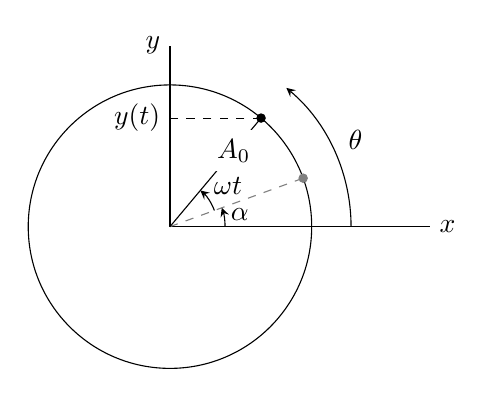
\begin{tikzpicture}
\pgfmathsetmacro{\angA}{20}
\pgfmathsetmacro{\angB}{50}
\pgfmathsetmacro{\rad}{1.8}
\pgfmathsetmacro{\xp}{\rad*cos(\angB)}
\pgfmathsetmacro{\yp}{\rad*sin(\angB)}
\draw[](0,0)--++(\rad+1.5,0)node[right]{$x$};
\draw[](0,0)--++(0,\rad+0.5)node[left]{$y$};
\draw[](0,0) circle (\rad);
\draw[gray,fill](\angA:\rad) circle (1.5pt);
\draw[fill](\angB:\rad) circle (1.5pt);
\draw[dashed,gray](0,0)--++(\angA:\rad);
\draw(0,0)--++(\angB:\rad)node[pos=0.7,fill=white]{$A_0$};
\draw[dashed](\xp,\yp)--(0,\yp)node[left]{$y(t)$};
%angles
\draw[-stealth] ([shift={(0:0.7)}]0,0) arc (0:\angA:0.7);
\draw(\angA/2:0.9)node{$\alpha$};
\draw[-stealth] ([shift={(\angA:0.6)}]0,0) arc (\angA:\angB:0.6);
\draw(\angA/2+\angB/2:0.9)node{$\omega t$};
\draw[-stealth] ([shift={(0:\rad+0.5)}]0,0) arc (0:\angB:\rad+0.5);
\draw(\angB/2:\rad+0.8)node{$\theta$};
\end{tikzpicture}
\caption*{(الف)}
\end{subfigure}%
\begin{subfigure}{0.5\textwidth}
\centering
\begin{tikzpicture}
\begin{axis}[kStyleCircuitsA,small,xlabel=$t$, ylabel=$y(t)$,ytick={1},yticklabels={$A_0$},xtick={180,360},xticklabels={$\pi$,$2\pi$},]
\addplot[domain=0:370,samples=100,dashed]{sin(x)}node[pos=0.42,pin={[font=\small]10:${A_0\sin \omega t}$},inner sep=0pt]{};
\addplot[domain=-60:320,samples=100]{sin(x+60)}node[pos=0.35,pin={[pin distance=0.75cm,font=\small]10:${A_0\sin (\omega t+\alpha)}$},inner sep=0pt]{};
\draw(axis cs:-60,-0.1)--(axis cs:-60,-0.3);
\draw[stealth-](axis cs:0,-0.2)--(axis cs:30,-0.2);
\draw[stealth-](axis cs:-60,-0.2)--(axis cs:-80,-0.2)--(axis cs:-80,-0.4)node[below]{$\alpha$};
\end{axis}
\end{tikzpicture}
\caption*{(ب) زاویائی ہٹاو۔}
\end{subfigure}%
\caption{لمحہ \عددی{t=0} پر زاویہ \عددی{\alpha} ہے۔}
\label{شکل_بدلتا_لمحہ_صفر_پر_مقام_الفا_ہے}
\end{figure}

زاویائی ہٹاو کو عموماً درجوں میں بیان کیا جاتا ہے لہٰذا \عددی{\alpha=\tfrac{\pi}{4}} کی صورت میں درج ذیل لکھا جا سکتا  ہے۔
\begin{align}\label{مساوات_بدلتا_زاویہ_ہٹاو_روایتی_طریقہ}
y(t)=A_0 \sin \left(\omega t +\frac{\pi}{4}\right)=A_0 \sin\left(\omega t+45^{\circ}\right)
\end{align}
با ضابطہ طور پر چونکہ \عددی{\omega t} کی قیمت ریڈیئن میں ہے لہٰذا \عددی{\alpha} کی قیمت بھی ریڈیئن میں ہونا لازم ہے لہٰذا تفاعل لکھنے کا صحیح طریقہ \عددی{y(t)=A_0\sin\left(\omega t+\tfrac{\pi}{4}\right)} ہی ہے لیکن زاویائی ہٹاو کو درجوں میں لکھنے کی روایت نہایت مقبول ہے لہٰذا اس کتاب میں بھی اس روایت کو برقرار رکھا جائے گا۔مساوات \حوالہ{مساوات_بدلتا_زاویہ_ہٹاو_روایتی_طریقہ} میں \عددی{45^{\circ}} لکھتے ہوئے زیر بالا میں درجے کی علامت \عددی{(^\circ)} استعمال کی گئی ہے جبکہ \عددی{\tfrac{\pi}{4}} پر کوئی علامت نہیں لگائی گئی۔اسی علامت سے ریڈیئن یا درجوں کی پہچان کی جاتی ہے۔
%================
\ابتدا{مثال}
مساوات \عددی{y_1(t)=15\sin(100t+60^{\circ})} اور \عددی{y_2(t)=22\sin(200t +0.2\pi)} کی قیمت \عددی{t=\SI{25}{\milli\second}} پر دریافت کریں۔

حل:پہلی تفاعل میں \عددی{50^{\circ}} کا زاویائی ہٹاو \عددی{\tfrac{60^{\circ}}{180^{\circ}}\times \pi=\tfrac{\pi}{3}} ریڈیئن کے برابر ہے۔یوں
 لمحہ \عددی{t=\SI{25}{\milli\second}} پر
\begin{align*}
y_1(0.025)&=15\sin\left(100\times 25\times 10^{-3}+\frac{\pi}{3}\right)=-5.918619766
\end{align*}
اور
\begin{align*}
y_2(0.025)&=22\sin(200\times 0.025+0.2\pi)=-13.39917888
\end{align*}
حاصل ہوتے ہیں۔
\انتہا{مثال}
%================== 

اگرچہ اب تک کی بحث میں ہم نے سائن تفاعل استعمال کیا، ہم اس کی جگہ کوسائن تفاعل بھی استعمال کر سکتے تھے۔ان دو تفاعل کی صورت بالکل یکساں ہے پس دونوں میں \عددی{90^{\circ}} کا زاویائی فرق پایا جاتا ہے۔
\begin{align}
\sin \left(\omega t+\frac{\pi}{2}\right)&=\cos \omega t\\
\cos \left(\omega t-\frac{\pi}{2}\right)&=\sin \omega t
\end{align}
سائن نما تفاعل کے دلیل  کے ساتھ \عددی{2\pi} ریڈیئن یا \عددی{360^{\circ}} کا مضرب جمع کرنے سے  تفاعل کی قیمت تبدیل نہیں ہوتی۔
\begin{align}
\cos(\omega t +\alpha+2\pi n)&=\cos(\omega t +\alpha) \quad \quad  n=0,\pm 1, \pm 2, \cdots \label{مساوات_بدلتا_طول_بعد_وہی_موج}\\
\sin(\omega t +\alpha+2\pi n)&=\sin(\omega t +\alpha) \quad \quad  n=0,\pm 1, \pm 2, \cdots \label{مساوات_بدلتا_طول_بعد_وہی_موج_ب}
\end{align}

دو سائن نما تفاعل میں زاویائی فرق  تین شرائط پورا کرنے کے بعد دریافت کیا جا سکتا ہے۔پہلی شرط یہ ہے کہ دونوں تفاعل کی تعدد برابر ہو۔دوسری شرط یہ ہے کہ دونوں کو  سائن تفاعل اور یا پھر دونوں کو  کوسائن تفاعل کی صورت میں لکھا جائے۔تیسری اور آخری شرط یہ ہے کہ دوسری شرط میں لکھے گئے تفاعل کے حیطے مثبت ہوں۔درج ذیل مماثل ان شرائط کو پورا کرنے میں مدد دیتے ہیں۔
\begin{align}
-\sin(\omega t+\alpha)&=\sin(\omega t+\alpha \pm 180^{\circ})\label{مساوات_بدلتا_آدھی_طول_منفی_موج_الف}\\
-\cos(\omega t+\alpha)&=\cos(\omega t+\alpha \pm 180^{\circ})\label{مساوات_بدلتا_آدھی_طول_منفی_موج_ب}
\end{align}
ان کے علاوہ درج ذیل مماثل بھی نہایت اہم ثابت ہوتے ہیں۔
\begin{align}
\sin(\alpha\pm\beta)&=\sin \alpha \cos \beta \pm \cos \alpha \sin \beta \label{مساوات_بدلتا_آدھی_طول_منفی_موج_پ}\\
\cos(\alpha \pm \beta)&=\cos \alpha \cos \beta \mp \sin \alpha \sin \beta \label{مساوات_بدلتا_آدھی_طول_منفی_موج_ت}
\end{align}
ایک آخری تفاعل جس کا ذکر ضروری ہے درج ذیل ہے۔
\begin{align} \label{مساوات_بدلتا_آدھی_طول_منفی_موج_ٹ}
\cos^2 \alpha+\sin^2 \alpha=1
\end{align}
%===============
\ابتدا{مثال}\شناخت{مثال_بدلتا_کوسائن_تفاعل_بالمقابل_ہٹاو}
درج ذیل تفاعل کے خط کھینچیں۔
\begin{itemize}
\item
$v(t)=1 \cos (\omega t +60^{\circ})$
\item
$v(t)=1 \cos (\omega t +240^{\circ})$
\item
$v(t)=1 \cos (\omega t -300^{\circ})$
\end{itemize}

حل: شکل \حوالہ{شکل_بدلتا_کوسائن_تفاعل_بالمقابل_ہٹاو}-الف میں \عددی{v(\omega t)=1\cos \omega t} کا خط دکھایا گیا ہے۔اس کو افقی محدد پر \عددی{60^{\circ}} درجے  بائیں منتقل کرنے سے \عددی{v(\omega t)=1\cos(\omega t +60^{\circ})} کا خط حاصل ہوتا ہے جسے شکل-ب میں دکھایا گیا ہے۔ ہم درج ذیل لکھ سکتے ہیں
\begin{align*}
v(\omega t)=1\cos (\omega t +240^{\circ})=1\cos (\omega t +60^{\circ}+180^{\circ})=-1\cos (\omega t +60^{\circ})
\end{align*}
جہاں مساوات \حوالہ{مساوات_بدلتا_آدھی_طول_منفی_موج_ب} کا استعمال کیا گیا ہے۔درج بالا مساوات کو شکل-پ میں دکھایا گیا ہے۔آپ دیکھ سکتے ہیں کہ یہ شکل-ب کا منفی ہے۔اسی طرح مساوات \حوالہ{مساوات_بدلتا_طول_بعد_وہی_موج} کی مدد سے
\begin{align*}
v(\omega t)=1\cos(\omega t-300^{\circ})=1\cos(\omega t-300^{\circ}+360^{\circ})=1\cos(\omega t+60^{\circ})
\end{align*}
لکھتے ہوئے شکل-ت حاصل ہوتی ہے جو عین شکل-ب ہی ہے۔
\begin{figure}
\centering
\begin{subfigure}{0.5\textwidth}
\centering
\begin{tikzpicture}
\begin{axis}[kStyleCircuitsA,small,xlabel=$\omega t$, ylabel=$v(\omega t)$,xtick={90,180,270,360}, xticklabels={$90^{\circ}$,$180^{\circ}$,$270^{\circ}$,$360^{\circ}$},ytick={-1,1},yticklabels={$-1$,$1$},]
\addplot[domain=0:360,samples=100]{1*cos(x)}node[pos=0.1,pin={[font=\small]10:${\cos \omega t}$},inner sep=0pt]{};
\end{axis}
\end{tikzpicture}
\caption*{(الف)}
\end{subfigure}%
\begin{subfigure}{0.5\textwidth}
\centering
\begin{tikzpicture}
\begin{axis}[kStyleCircuitsA,small,xlabel=$\omega t$, ylabel=$v(\omega t)$,xtick={-60,30,120,210,300}, xticklabels={$-60^{\circ}$,$30^{\circ}$,$120^{\circ}$,$210^{\circ}$,$300^{\circ}$},ytick={-1,1},yticklabels={$-1$,$1$},]
\addplot[domain=-60:300,samples=100]{1*cos(x+60)}node[pos=0.85,pin={[font=\small]170:${\cos (\omega t+60^{\circ})}$},inner sep=0pt]{};
\end{axis}
\end{tikzpicture}
\caption*{(ب)}
\end{subfigure}
\begin{subfigure}{0.5\textwidth}
\centering
\begin{tikzpicture}
\begin{axis}[kStyleCircuitsA,small,xlabel=$\omega t$, ylabel=$v(\omega t)$,xtick={-60,30,120,210,300},
 xticklabels={$-60^{\circ}$,$30^{\circ}$,$120^{\circ}$,$210^{\circ}$,$300^{\circ}$},ytick={-1,1},yticklabels={$-1$,$1$},]
\addplot[domain=-60:300,samples=100]{1*cos(x+240)}node[pos=0.85,pin={[font=\small]-170:${\cos( \omega t+240^{\circ})}$},inner sep=0pt]{};
\end{axis}
\end{tikzpicture}
\caption*{(پ)}
\end{subfigure}%
\begin{subfigure}{0.5\textwidth}
\centering
\begin{tikzpicture}
\begin{axis}[kStyleCircuitsA,small,xlabel=$\omega t$, ylabel=$v(\omega t)$,xtick={-60,30,120,210,300}, 
xticklabels={$-60^{\circ}$,$30^{\circ}$,$120^{\circ}$,$210^{\circ}$,$300^{\circ}$},ytick={-1,1},yticklabels={$-1$,$1$},]
\addplot[domain=-60:300,samples=100]{1*cos(x-300)}node[pos=0.85,pin={[font=\small]170:${\cos( \omega t-300^{\circ})}$},inner sep=0pt]{};
\end{axis}
\end{tikzpicture}
\caption*{(ت)}
\end{subfigure}%
\caption{مثال \حوالہ{مثال_بدلتا_کوسائن_تفاعل_بالمقابل_ہٹاو} کے خط۔}
\label{شکل_بدلتا_کوسائن_تفاعل_بالمقابل_ہٹاو}
\end{figure}
\انتہا{مثال}
%==========================
\ابتدا{مثال}
درج ذیل امواج کی تعدد ہرٹز میں حاصل کریں۔ امواج کے مابین زاویائی فرق دریافت کریں۔یہ بھی بتلائیں کہ کونسی موج آگے ہے۔
\begin{align*}
v_1(\omega t)&=100\sin(400t -30^{\circ})\\
v_2(\omega t)&=-250\cos(400t+0.2\pi)
\end{align*}

حل:ان امواج میں \عددی{\omega=\SI{400}{\radian\per\second}} ہے لہٰذا
\begin{align*}
f=\frac{\omega}{2\pi}=\frac{400}{2\pi}=\SI{63.66}{\hertz}
\end{align*}
ہو گا۔زاویائی فرق دریافت کرنے کی خاطر دونوں امواج کو مثبت حیطے کے کوسائن موج کی صورت میں لکھتے ہیں۔ساتھ ہی ساتھ ان کے زاویائی ہٹاو کو درجوں میں لکھتے ہیں۔یوں
\begin{align*}
v_1(\omega t)&=100\sin(400t -30^{\circ})\\
&=100\cos(400t-30^{\circ}-90^{\circ})\\
&=100\cos(400t-120^{\circ})\\
&=100\cos(400t+240^{\circ})
\end{align*}
لکھا جا سکتا ہے جہاں آخری قدم پر مساوات \حوالہ{مساوات_بدلتا_طول_بعد_وہی_موج} کا استعمال کیا گیا۔اسی طرح
\begin{align*}
v_2(\omega t)&=-250\cos(400t+0.2\pi)\\
&=250\cos(400t+0.2\pi+\pi)\\
&=250\cos(400t+216^{\circ})
\end{align*}
بھی لکھا جا سکتا ہے جہاں آخری قدم پر \عددی{1.2\pi} ریڈیئن کو \عددی{216^{\circ}} درجے لکھا گیا ہے۔ان امواج کے مابین
\begin{align*}
240^{\circ}-216^{\circ}=24^{\circ}
\end{align*}
کا زاویائی فرق پایا جاتا ہے اور موج \عددی{v_1(\omega t)} آگے ہے۔
\انتہا{مثال}
%========================
\ابتدا{مشق}
ایک دور میں درج ذیل تین رو پائے جاتے ہیں۔
\begin{align*}
i_1(1)&=30\cos(100\pi t+30^{\circ})\\
i_2(2)&=55\sin(100\pi t +40^{\circ})\\
i_3(t)&=20\sin(100 \pi t+60^{\circ})
\end{align*}
\عددی{i_2} سے \عددی{i_1} کتنی آگے ہے اور \عددی{i_3} سے \عددی{i_1} کتنی پیچھے ہے۔

جوابات:\عددی{80^{\circ}}، \عددی{-60^{\circ}} یا \عددی{300^{\circ}} 
\انتہا{مشق}
%=========================
\حصہ{سائن نما اور مخلوط جبری تفاعل}
گزشتہ باب میں دور پر مستقل جبری تفاعل مسلط  کرتے ہوئے، دور کا جبری ردعمل بھی مستقل قیمت کا حاصل ہوا۔تفرقی مساوات کا جبری ردعمل، مسلط جبری تفاعل اور اس کے تمام بلند درجی تفرق کا مجموعہ ہوتا ہے۔یوں  دور پر جبری دباو \عددی{v(t)=\sin \omega t} مسلط کرنے سے رو کا جبری ردعمل \عددی{i(t)=c_1\sin\omega t+c_2\cos\omega t} متوقع ہو گا۔پس جبری ردعمل کے مستقل \عددی{c_1} اور \عددی{c_2} معلوم کرنا باقی ہے۔
%===============
\ابتدا{مثال}\شناخت{مثال_بدلتا_مزاحمت_امالہ_جبری_حل_الف}
شکل \حوالہ{شکل_بدلتا_مزاحمت_امالہ_جبری_حل_الف} میں رو \عددی{i_J(t)} حاصل کریں۔

\begin{figure}
\centering
\begin{tikzpicture}
\draw(0,0) to [american voltage source,l={${v(t)=V_0\cos \omega t}$}]++(0,\y) to [resistor,i={$i(t)$},l={$R$}]++(\x,0) to [inductor,l={$L$}]++(0,-\y) to [short] (0,0);
\end{tikzpicture}
\caption{مثال \حوالہ{مثال_بدلتا_مزاحمت_امالہ_جبری_حل_الف} کا دور۔}
\label{شکل_بدلتا_مزاحمت_امالہ_جبری_حل_الف}
\end{figure}

حل: دور کی تفرقی مساوات لکھتے ہیں۔
\begin{align}\label{مساوات_بدلتا_مزاحمت_امالہ_جبری_حل_الف}
R i(t)+L \frac{\dif i(t)}{\dif t}=V_0 \cos \omega t
\end{align}
دور پر مسلط جبری تفاعل اور اس تفاعل کے تمام بلند درجی تفرق کا مجموعہ جبری حل کے برابر ہو گا۔
\begin{align*}
i_J(t)&=c_1 \cos \omega t+c_2\sin \omega t
\end{align*} 
اس جبری حل کو مساوات \حوالہ{مساوات_بدلتا_مزاحمت_امالہ_جبری_حل_الف} میں پُر کرتے ہوئے \عددی{c_1} اور \عددی{c_2} مستقل دریافت کرتے ہیں۔ 
\begin{align*}
R(c_1 \cos \omega t+c_2\sin \omega t)+L (-c_1 \omega \sin\omega t+c_2 \omega \cos \omega t)=V_0 \cos \omega t
\end{align*}
درج بالا مساوات میں دونوں اطراف \عددی{\cos \omega t} کے  عددی سر برابر ہوں گے۔اسی طرح دونوں اطراف \عددی{\sin \omega t} کے عددی سر برابر ہوں گے۔
\begin{align*}
c_1 R+c_2 \omega L&=V_0\\
-c_1 \omega L+c_2 R&=0
\end{align*}
ان ہمزاد مساوات کو \عددی{c_1} اور \عددی{c_2} کے لئے حل کرتے ہوئے درج ذیل ملتا ہے
\begin{align*}
c_1&=\frac{R V_0}{R^2+\omega^2 L^2}\\
c_2&=\frac{\omega L V_0}{R^2+\omega^2 L^2}
\end{align*}
لہٰذا جبری حل
\begin{align}\label{مساوات_بدلتا_جبری_حل_الف}
i_J(t)=\frac{R V_0}{R^2+\omega^2 L^2} \cos \omega t+\frac{\omega L V_0}{R^2+\omega^2 L^2} \sin \omega t
\end{align}
ہو گا۔
\انتہا{مثال}
%=================
\ابتدا{مثال}\شناخت{مثال_بدلتا_مزاحمت_امالہ_جبری_حل_ب}
درج بالا مثال میں \عددی{R=\SI{100}{\ohm}}، \عددی{L=\SI{5}{\milli\henry}}، \عددی{V_0=\SI{310}{\volt}} اور \عددی{\omega=\SI{10}{\kilo\radian\per\second}} کی صورت میں جبری حل کو مساوات \حوالہ{مساوات_بدلتا_آدھی_طول_منفی_موج_ت} کی مدد سے \عددی{i(t)=I_0\cos(\omega t-\phi)} کے طرز پر لکھیں۔

حل: مساوات \حوالہ{مساوات_بدلتا_جبری_حل_الف} میں دی گئی قیمتیں پُر کرنے سے
\begin{align*}
i_J(t)&=\frac{100\times 310}{100^2+(\num{10000}\times 0.005)^2} \cos \omega t+\frac{\num{10000}\times 0.005\times 310}{100^2+(\num{10000}\times 0.005)^2} \sin \omega t
\end{align*}
یعنی درج ذیل حاصل ہوتا ہے۔
\begin{align}\label{مساوات_بدلتا_جبری_حل_ب}
i_J(t)=2.48\cos \omega t+1.24\sin \omega t
\end{align}
مساوات \حوالہ{مساوات_بدلتا_آدھی_طول_منفی_موج_ت} سے  جبری حل کی درکار صورت کو درج ذیل لکھا جا سکتا ہے۔ 
\begin{align}\label{مساوات_بدلتا_جبری_حل_پ}
i(t)=I_0 \cos(\omega t-\phi)=I_0 \cos \phi \cos \omega t+I_0 \sin \phi \sin \omega t
\end{align}
مساوات \حوالہ{مساوات_بدلتا_جبری_حل_ب} میں \عددی{\cos \omega t} اور \عددی{\sin \omega t} کے عددی سر کو مساوات \حوالہ{مساوات_بدلتا_جبری_حل_پ} کے عددی سر کے برابر پُر کرتے ہیں۔
\begin{align}
I_0 \cos \phi &=2.48 \label{مساوات_بدلتا_جبری_حل_ت}\\
I_0 \sin \phi&=1.24 \label{مساوات_بدلتا_جبری_حل_ٹ}
\end{align}
ان ہمزاد مساوات کے مربع جمع کرتے ہوئے 
\begin{align*}
I_0^2 \cos^2 \phi+I_0^2 \sin^2 \phi=2.48^2+1.24^2
\end{align*}
ملتا ہے جس میں مساوات \حوالہ{مساوات_بدلتا_آدھی_طول_منفی_موج_ٹ} کے استعمال سے  \عددی{\cos^2 \phi+\sin^2 \phi=1} پُر کرتے ہوئے
\begin{align*}
I_0=\sqrt{2.48^2+1.24^2}=2.7727
\end{align*}
ملتا ہے۔اسی طرح مساوات \حوالہ{مساوات_بدلتا_جبری_حل_ٹ} کو مساوات \حوالہ{مساوات_بدلتا_جبری_حل_ت} سے تقسیم کرنے سے
\begin{align*}
\frac{\sin \phi}{\cos \phi}=\frac{1.24}{2.48}=\tan \phi
\end{align*}
یعنی
\begin{align*}
\phi=\tan ^{-1}\frac{1.24}{2.48}=\phase{26.6^{\circ}}
\end{align*}
ملتا ہے۔یوں جبری حل درج ذیل لکھا جائے گا
\begin{align}
i_J(t)=2.77\cos(\omega t-26.6^{\circ})=2.77\cos(\num{10000} t-26.6^{\circ})
\end{align}
جہاں سے ظاہر ہے کہ دباو سے رو \عددی{26.6^{\circ}} درجے پیچھے ہے۔ مخلوط جبری حل درج ذیل لکھا جائے گا جس کا حقیقی جزو درج بالا مساوات ہے۔
\begin{align}\label{مساوات_بدلتا_مخلوط_رو_صورت}
i_M(t)=2.77 e^{j(\num{10000} t-26.6^{\circ})}
\end{align}
\انتہا{مثال}
%===================
\ابتدا{مثال}\شناخت{مثال_بدلتا_مزاحمت_امالہ_جبری_حل_پ}
مثال \حوالہ{مثال_بدلتا_مزاحمت_امالہ_جبری_حل_ب} کے طرز پر مثال \حوالہ{مثال_بدلتا_مزاحمت_امالہ_جبری_حل_الف} میں حاصل کئے گئے جبری حل کو \عددی{i_J(t)=I_0\cos(\omega t -\phi)} کی صورت میں لکھیں۔

حل:مساوات \حوالہ{مساوات_بدلتا_جبری_حل_الف} میں \عددی{\cos \omega t} اور \عددی{\sin \omega t} کے عددی سر کو مساوات \حوالہ{مساوات_بدلتا_جبری_حل_پ} میں \عددی{\cos \omega t} اور \عددی{\sin \omega t} کے عددی سر کے برابر پُر کرتے ہوئے درج ذیل ملتا ہے۔
\begin{align*}
I_0 \cos \phi&=\frac{R V_0}{R^2+\omega^2 L^2}\\
I_0 \sin \phi&=\frac{\omega L V_0}{R^2+\omega^2 L^2}
\end{align*}
ان ہمزاد مساوات میں دوسری مساوات کو پہلی سے تقسیم کرتے ہوئے
\begin{align*}
\frac{\sin \phi}{\cos \phi}=\tan \phi=\frac{\omega L}{R}
\end{align*}
یعنی
\begin{align}
\phi=\tan^{-1}{\frac{\omega L}{R}}
\end{align}
ملتا ہے جبکہ دونوں ہمزاد مساوات کے مربع کا مجموعہ لیتے ہوئے
\begin{align*}
I_0^2 \cos^2 \phi+I_0^2 \sin^2 \phi=I_0^2&=\left(\frac{R V_0}{R^2+\omega^2 L^2}\right)^2+\left(\frac{\omega L V_0}{R^2+\omega^2 L^2}\right)^2 \\
&=\frac{(R^2+\omega^2 L^2)V_0^2}{(R^2+\omega^2 L^2)^2}\\
&=\frac{V_0^2}{R^2+\omega^2 L^2}
\end{align*}
یعنی
\begin{align}
I_0=\frac{V_0}{\sqrt{R^2+\omega^2 L^2}}
\end{align}
ملتا ہے۔یوں جبری حل درج ذیل لکھا جائے گا۔
\begin{align}\label{مساوات_بدلتا_جبری_حل_امالہ_مزاحمت}
i_J(t)=\frac{V_0}{\sqrt{R^2+\omega^2 L^2}} \cos \left(\omega t -\tan^{-1}{\frac{\omega L}{R}}\right)
\end{align}
\انتہا{مثال}
%========================

مساوات \حوالہ{مساوات_بدلتا_جبری_حل_امالہ_مزاحمت} سے ظاہر ہے کہ \عددی{L=0} کی صورت میں \عددی{\phi=0} ہو گا لہٰذا دباو اور رو ہم زاویہ ہوں گے جبکہ \عددی{R=0} کی صورت میں \عددی{\phi=90^{\circ}} ہو گا لہٰذا دباو سے رو \عددی{90^{\circ}} درجے پیچھے ہو گی۔مزاحمت اور امالہ کے دیگر قیمتوں کی صورت میں دباو سے رو \عددی{0^{\circ}} تا \عددی{90^{\circ}} کے مابین کسی مخصوص  درجے پر پیچھے رہے گی۔اسی لئے مزاحمت اور امالہ کے ادوار کو پیچھے رہنے والے ادوار کہا جاتا ہے۔

سلسلہ وار جڑے مزاحمت اور امالہ کے دور کا حل آپ نے دیکھا۔یقیناً اس دور کا حل سلسلہ وار جڑے دو عدد مزاحمتی دور کے حل سے کئی گنا مشکل تھا۔آپ خود تصور کر سکتے ہیں کہ زیادہ تعداد کے پرزوں کا دور حل کرنا کتنا مشکل ہو گا۔اسی مشکل کو مد نظر رکھتے ہوئے ہم \اصطلاح{مخلوط تفاعل}\فرہنگ{مخلوط تفاعل}\حاشیہب{complex function}\فرہنگ{complex function} کو پیش کرتے ہیں جس سے ادوار کا حل انتہائی آسان ثابت ہوتا ہے۔

مخلوط تفاعل اور سائن نما تفاعل کا تعلق \اصطلاح{یولر مساوات}\فرہنگ{یولر مساوات}\حاشیہب{Euler's equation}\فرہنگ{Euler's equation}
\begin{align}
e^{j\omega t}=\cos \omega t +j \sin \omega t \quad \quad \text{\RL{یولر مساوات}}
\end{align}
دیتی ہے جہاں \عددی{j=\sqrt{-1}} خیالی عدد ہے۔یولر مساوات میں \عددی{\cos \omega t} \اصطلاح{حقیقی}\فرہنگ{حقیقی}\حاشیہب{real}\فرہنگ{real} مقدار اور \عددی{\sin \omega t} \اصطلاح{خیالی}\فرہنگ{خیالی}\حاشیہب{imaginary}\فرہنگ{imaginary} مقدار ہیں۔

حقیقی دنیا میں مخلوط جبری تفاعل نہیں پایا جاتا۔اس کے باوجود، دور پر سائن نما جبری تفاعل کی جگہ مخلوط جبری تفاعل مسلط کرتے ہوئے  مخلوط حل حاصل کیا جا سکتا ہے۔مخلوط جبری تفاعل کو حقیقی جبری تفاعل اور خیالی جبری تفاعل کا مجموعہ تصور کیا جا سکتا ہے۔خطی ادوار میں مسئلہ نفاذ کے تحت تمام جبری تفاعل کی علیحدہ علیحدہ اثرات کا مجموعہ لیا جا سکتا ہے۔یوں جبری تفاعل کے حقیقی جزو سے حل کا حقیقی جزو جبکہ جبری تفاعل کے خیالی جزو سے حل کا خیالی جزو حاصل ہو گا۔یوں مخلوط حل کے خیالی جزو کو رد کرتے ہوئے حقیقی جزو کو سائن نما تفاعل کا ردعمل تسلیم کیا جاتا ہے۔اس ترکیب کو مثال کی مدد سے زیادہ آسانی سے سمجھا جا سکتا ہے۔
%====================
\ابتدا{مثال}\شناخت{مثال_بدلتا_مخلوط_تفاعل_الف}
شکل \حوالہ{شکل_بدلتا_مزاحمت_امالہ_جبری_حل_الف} میں حقیقی جبری تفاعل \عددی{V_0\cos \omega t} کی جگہ مخلوط جبری تفاعل نسب کرتے ہوئے حقیقی \عددی{i(t)} کے لئے حل کریں۔

حل:حقیقی جبری تفاعل \عددی{v(t)=V_0\cos \omega t} کی جگہ دور میں مخلوط جبری تفاعل \عددی{v(t)=V_0 e^{j\omega t}} نسب کرتے ہوئے کرخوف مساوات لکھتے ہیں۔
\begin{align*}
R i(t) +L\frac{\dif i(t)}{\dif t}=V_0 e^{j \omega t}
\end{align*}
جبری تفاعل \عددی{e^{j\omega t}} کا تفرق \عددی{j\omega e^{j\omega t}} بھی جبری تفاعل ہی ہے لہٰذا درج بالا مساوات کا مخلوط حل \عددی{i_M(t)=I_0e^{j\omega t}} فرض  کرتے ہیں جہاں \عددی{I_0} نا معلوم مخلوط مستقل ہے۔اس حل کو درج بالا مساوات میں پُر کرتے ہوئے
\begin{align*}
R I_0 e^{j\omega t}+L \frac{\dif}{\dif t}\left(I_0 e^{j\omega t} \right)=V_0 e^{j \omega t}
\end{align*}
درکار تفرق کے بعد
\begin{align}\label{مساوات_بدلتا_مخلوط_الف}
R I_0  e^{j \omega t}+j \omega L I_0e^{j\omega t}&=V_0 e^{j \omega t}
\end{align}
ملتا ہے جس کے دونوں اطراف کو \عددی{e^{j\omega t}} سے تقسیم کرتے ہوئے درج ذیل ملتا ہے۔
\begin{align}\label{مساوات_بدلتا_مخلوط_ب}
R I_0+j \omega L I_0&=V_0 
\end{align}
اس سے \عددی{I_0} حاصل کرتے ہیں۔
\begin{align}\label{مساوات_بدلتا_مخلوط_مستقل_الف}
I_0=\frac{V_0}{R+j\omega L}
\end{align}
یوں مخلوط رو درج ذیل لکھی جا سکتی ہے۔
\begin{gather}
\begin{aligned}\label{مساوات_بدلتا_مخلوط_پ}
i_M(t)&=I_0 e^{j\omega t}\\
&=\frac{V_0 e^{j\omega t}}{R+j\omega L}
\end{aligned}
\end{gather}
ہمیں اس کا حقیقی جزو درکار ہے۔یولر مساوات کی مدد سے درج بالا مساوات کو درج ذیل لکھا جا سکتا ہے۔
\begin{align*}
i_M(t)&=\frac{V_0 (\cos \omega t+j \sin \omega t)}{R+j\omega L}
\end{align*}
دائیں ہاتھ کسر کے بالائی اور نچلے حصے کو \عددی{R-j\omega t} سے ضرب دیتے ہیں
 \begin{align*}
i_M(t)&=\frac{V_0 (\cos \omega t+j \sin \omega t)(R-j\omega L)}{(R+j\omega L)(R-j\omega L)}\\
&=\frac{V_0(R \cos \omega t+\omega L \sin \omega t)+jV_0(R\sin \omega t-\omega L \cos \omega t)}{R^2+\omega^2 L^2}
\end{align*}
جہاں دوسرا قدم ترتیب دیتے ہوئے لکھا گیا ہے۔اس کا حقیقی جزو درکار حل ہے
\begin{align}\label{مساوات_بدلتا_مخلوط_ت}
i(t)=\frac{V_0(R \cos \omega t+\omega L \sin \omega t)}{R^2+\omega^2 L^2}
\end{align}
جو عین مساوات \حوالہ{مساوات_بدلتا_جبری_حل_الف} ہی ہے۔

ہم مساوات \حوالہ{مساوات_بدلتا_مخلوط_مستقل_الف} کے مخلوط مستقل \عددی{I_0} کو زاویائی شکل میں لکھ کر بھی آگے بڑھ سکتے ہیں۔مخلوط مستقل کو درج ذیل لکھا جا سکتا ہے
\begin{align*}
I_0&=\frac{V_0}{R+j\omega L}\\
&=\frac{V_0}{\sqrt{R^2+\omega^2 L^2} \phase{\tan^{-1}\frac{\omega L}{R}}}\\
&=\frac{V_0}{\sqrt{R^2+\omega^2 L^2}\,  e^{j\tan^{-1}\frac{\omega L}{R}}}\\
&=\frac{V_0}{\sqrt{R^2+\omega^2 L^2}} e^{-j\tan^{-1}\frac{\omega L}{R}}
\end{align*}
جہاں دوسری قدم پر کسر کے نچلی حصے کو مساوات \حوالہ{مساوات_بدلتا_مستطیل_سے_زاویائی} کی مدد سے زاویائی صورت میں لکھا گیا ہے اور تیسری قدم پر یولر مساوات کا استعمال کیا گیا ہے۔زاویہ \عددی{\theta=\tan^{-1} \tfrac{\omega L}{R}} کو شکل \حوالہ{شکل_بدلتا_مخلوط_تفاعل_الف} میں دکھایا گیا ہے۔ یوں مخلوط رو درج ذیل لکھی جائے گی۔
\begin{align*}
i_M&=I_0 e^{j\omega t}\\
&=\frac{V_0}{\sqrt{R^2+\omega^2 L^2}} e^{j\left(\omega t-\tan^{-1}\frac{\omega L}{R}\right)} 
\end{align*}
اس مساوات میں \عددی{\tan^{-1}\tfrac{\omega L}{R}=\theta} لکھتے ہوئے حقیقی جزو لے کر حقیقی رو حاصل کرتے ہیں۔
\begin{align*}
i(t)&=\left. \frac{V_0}{\sqrt{R^2+\omega^2 L^2}} e^{j\left(\omega t-\theta\right)} \right|_{\text{حقیقی}} \\
&=\frac{V_0}{\sqrt{R^2+\omega^2 L^2}} \cos (\omega t-\theta)\\
&=\frac{V_0}{\sqrt{R^2+\omega^2 L^2}} \left(\cos \omega t \cos \theta+\sin \omega t \sin \theta \right)
\end{align*}
شکل \حوالہ{شکل_بدلتا_مخلوط_تفاعل_الف} سے  \عددی{\cos \theta=\tfrac{R}{\sqrt{R^2+\omega^2L^2}}} اور
 \عددی{\sin \theta=\tfrac{\omega L}{\sqrt{R^2+\omega^2L^2}}} پُر کرتے ہوئے
\begin{align*}
i(t)&=\frac{V_0}{\sqrt{R^2+\omega^2 L^2}} \left(\cos \omega t \frac{R}{\sqrt{R^2+\omega^2 L^2}}+\sin \omega t \frac{\omega L}{\sqrt{R^2+\omega^2 L^2}}\right)\\
&=\frac{V_0 (R \cos \omega t +\omega L \sin \omega t)}{R^2+\omega^2 L^2}
\end{align*}
%
\begin{figure}
\centering
\begin{tikzpicture}
\pgfmathsetmacro{\l}{3};
\pgfmathsetmacro{\ang}{20};
\pgfmathsetmacro{\x}{\l*cos(\ang)};
\pgfmathsetmacro{\y}{\l*sin(\ang)};
\draw(0,0)--++(4,0)node[right]{حقیقی};
\draw(0,0)--++(0,1.5)node[left]{خیالی};
\draw(0,0)--++(\ang:\l)coordinate(kp)node[pos=0.5,above,sloped]{$\sqrt{R^2+\omega^2 L^2}$};
\draw(\x,0)--(kp)node[pos=0.5,right]{$\omega L$};
\draw(\x/2,0)node[below]{$R$};
\draw[-stealth]([shift={(0:0.8)}]0,0) arc (0:\ang:0.8);
\draw(\ang/2:1)node{$\theta$};
\end{tikzpicture}
\caption{مثال \حوالہ{مثال_بدلتا_مخلوط_تفاعل_الف} کا شکل۔}
\label{شکل_بدلتا_مخلوط_تفاعل_الف}
\end{figure}
\انتہا{مثال}
%================

\حصہ{دوری سمتیہ}
درج بالا حصے میں ہم نے دیکھا کہ حقیقی جبری تفاعل کی جگہ مخلوط جبری تفاعل نسب کرتے ہوئے مخلوط حل حاصل کیا جا سکتا ہے جس کا حقیقی جزو حقیقی جبری رد عمل ہو گا۔ اس ترکیب کو مثال \حوالہ{مثال_بدلتا_مخلوط_تفاعل_الف} میں استعمال کیا گیا جہاں مساوات \حوالہ{مساوات_بدلتا_مخلوط_الف} کو \عددی{e^{j\omega t}} سے تقسیم کرتے ہوئے مساوات \حوالہ{مساوات_بدلتا_مخلوط_ب} حاصل کی گئی۔ مساوات \حوالہ{مساوات_بدلتا_مخلوط_ب} سے \عددی{I_0} حاصل کی گئی جسے  \عددی{e^{j\omega t}} سے ضرب دیتے ہوئے مخلوط حل حاصل کیا گیا۔مخلوط حل کا حقیقی جزو یعنی مساوات \حوالہ{مساوات_بدلتا_مخلوط_ت} درکار جواب ہے۔مثال \حوالہ{مثال_بدلتا_مزاحمت_امالہ_جبری_حل_ب} میں  مخصوص قیمتیں استعمال کرتے  ہوئے مخلوط رو کو مساوات \حوالہ{مساوات_بدلتا_مخلوط_رو_صورت}  میں پیش کیا گیا۔آپ دیکھ سکتے ہیں کہ جزو \عددی{e^{j \omega t}}  جوں کا توں مخلوط جبری تفاعل اور مخلوط جبری حل میں پایا جاتا ہے۔

حقیقت میں کسی بھی خطی دور پر مخلوط جبری تفاعل مثلاً
\begin{align}
v_M=V_0 e^{j \omega t}
\end{align}
مسلط کرنے سے دور میں تمام رو کی صورت \عددی{i_M(t)=I_0e^{j(\omega t+\phi)}} اور دباو کی صورت \عددی{v_M(t)=V_0e^{j(\omega t+\phi)}} ہو گی جہاں تمام رو اور دباو  کی تعدد \عددی{\omega} جبکہ ان کے انفرادی  حیطے \عددی{I_0} یا \عددی{V_0} اور زاویہ ہٹاو \عددی{\phi} مختلف ہوں گے۔یہاں حیطہ حقیقی مقدار ہے۔

یوں تعدد جانتے ہوئے کسی بھی مخلوط تفاعل مثلاً مخلوط رو کو اس کے حیطے \عددی{I_0} اور زاویائی ہٹاو \عددی{\phi} سے مکمل طور پر ظاہر کیا جا سکتا ہے۔مخلوط تفاعل مثلاً 
\begin{align}
i_M(t)=I_0 e^{j(\omega t+\phi)}
\end{align}
سے حقیقی تفاعل درج ذیل
\begin{align}\label{مساوات_بدلتا_حقیقی_رو_الف}
i(t)&=\left. I_0 e^{j(\omega t+\phi)} \right|_{\text{حقیقی}}
\end{align}
لکھا جا سکتا ہے جہاں \عددی{I_0} حقیقی مقدار ہے اور زیر نوشت میں لفظ "حقیقی" لکھنے کا مطلب ہے کہ اس تفاعل کا حقیقی جزو لیا جائے یعنی
\begin{align}\label{مساوات_بدلتا_حقیقی_رو_ب}
i(t)&=I_0 \cos (\omega t+\phi)
\end{align}
مساوات \حوالہ{مساوات_بدلتا_حقیقی_رو_الف} حقیقی رو دیتی ہے۔اس طرز کے تمام مساوات میں \عددی{e^{j\omega t}} پایا جاتا ہے اور مساوات کا حقیقی جزو ہی حقیقی مقدار ہوتا ہے۔یوں ایسے مساوات میں لفظ "حقیقی" اور \عددی{e^{j\omega t}} کو ذہن میں رکھتے ہوئے انہیں لکھنے سے گریز کیا جاتا ہے۔مساوات \حوالہ{مساوات_بدلتا_حقیقی_رو_الف} میں ایسا ہی کرتے ہوئے درج ذیل لکھا جائے گا
\begin{align}\label{مساوات_بدلتا_دوری_سمتیہ_الف}
\hat{I}=I_0e^{j\phi}
\end{align}
جہاں رو کو ٹوپی والے بڑے حرف سے ظاہر کیا گیا ہے۔دباو کی صورت میں تفاعل کو \عددی{\hat{V}} لکھا جاتا۔ٹوپی والے بڑے حرف سے ظاہر کردہ تفاعل کو \عددی{e^{j\omega t}} سے ضرب دے کر حقیقی جزو لینے سے حقیقی تفاعل حاصل کیا جاتا ہے۔

مساوات \حوالہ{مساوات_بدلتا_دوری_سمتیہ_الف} کا صفحہ \حوالہصفحہ{مساوات_بدلتا_مخلوط_عدد_طرز_لکھائی} پر مساوات \حوالہ{مساوات_بدلتا_مخلوط_عدد_طرز_لکھائی} سے موازنہ کریں۔ایسا معلوم ہوتا ہے جیسے  \عددی{\hat{I}} مخلوط عدد کو ظاہر کرتا ہے۔اگرچہ مساوات \حوالہ{مساوات_بدلتا_دوری_سمتیہ_الف} درحقیقت میں مساوات \حوالہ{مساوات_بدلتا_حقیقی_رو_الف} کو چھوٹا لکھنے کا طریقہ ہے لہٰذا \عددی{\hat{I}} مخلوط عدد کو ظاہر نہیں کرتا لیکن دیکھا یہ گیا ہے کہ \عددی{\hat{I}} کو مخلوط عدد تصور کر لینے سے ہمارے لئے آسانی پیدا ہوتی ہے۔آئیں \عددی{\hat{V}} کو مخلوط عدد فرض کرتے ہوئے اس کو مخلوط سطح پر ظاہر کریں۔
%=========================== 
\ابتدا{مثال}\شناخت{مثال_بدلتا_دوری_سمتیہ_مثال_الف}
مخلوط دباو \عددی{v_M(t)=50e^{j(100\pi t-35^{\circ})}}سے \عددی{\hat{V}} حاصل کرتے ہوئے \عددی{\hat{V}} کو مخلوط سطح پر دکھائیں۔

حل:مخلوط دباو سے حقیقی دباو لکھتے ہیں۔
\begin{align*}
v(t)=\left. 50e^{j(100\pi t-35^{\circ})} \right|_{\text{حقیقی}}
\end{align*}
اس مساوات کی تعدد \عددی{(\omega=100\pi)} کو ذہن نشین کرتے ہوئے لفظ "حقیقی" اور \عددی{e^{j100\pi t}} لکھنے سے گریز کرتے ہوئے درج ذیل لکھا جائے گا
\begin{align*}
\hat{V}&=50e^{-j35^{\circ}}\\
&=50\phase{-35^{\circ}}
\end{align*}
جسے شکل \حوالہ{شکل_بدلتا_دوری_سمتیہ_مثال_الف} میں مخلوط سطح پر دکھایا گیا ہے۔حقیقی محدد سے گھڑی کی گردش کی جانب مثبت زاویہ ناپا جاتا ہے لہٰذا منفی زاویے کو گھڑی کی گردش کے الٹ جانب دکھایا گیا ہے۔مخلوط اعداد اور \عددی{\hat{V}} میں فرق رکھنے کی خاطر \عددی{\hat{V}} کو مخلوط سطح پر تیر کی نشان سے ظاہر کیا جاتا ہے۔
\begin{figure}
\centering
\begin{tikzpicture}
\draw(0,0)--++(3,0)node[right]{حقیقی};
\draw(0,-1.5)--(0,0.5)node[left]{خیالی};
\draw[-latex] (0,0)--++(-35:2.5)node[right]{$\hat{V}$}node[pos=0.6,below left]{$50$};
\draw[-stealth]([shift={(0:0.5)}]0,0) arc (0:-35:0.5);
\draw(-35*2/3:0.6)node[right]{$35^{\circ}$};
\end{tikzpicture}
\caption{مثال \حوالہ{مثال_بدلتا_دوری_سمتیہ_مثال_الف} کی دوری سمتیہ۔}
\label{شکل_بدلتا_دوری_سمتیہ_مثال_الف}
\end{figure}
\انتہا{مثال}
%===========================

مثال \حوالہ{مثال_بدلتا_دوری_سمتیہ_مثال_الف} میں \عددی{\hat{V}} کو مخلوط سطح پر تیر کے نشان سے ظاہر کیا گیا ہے جسے دیکھ کر یوں معلوم ہوتا ہے جیسے \عددی{\hat{V}} ایک سمتیہ ہے۔اسی حقیقت کی بنا پر \عددی{\hat{V}} یا \عددی{\hat{I}} کو \اصطلاح{دوری سمتیہ}\فرہنگ{دوری سمتیہ}\حاشیہب{phasor}\فرہنگ{phasor} کہتے ہیں اور شکل \حوالہ{شکل_بدلتا_دوری_سمتیہ_مثال_الف} کو \اصطلاح{دوری سمتی شکل}\فرہنگ{دوری سمتی شکل}\حاشیہب{phasor diagram}\فرہنگ{phasor diagram} کہتے ہیں۔

مخلوط عدد لکھنے کے تمام طرز پر دوری سمتیہ کو لکھا جاتا ہے لہٰذا درج ذیل لکھنا ممکن ہے۔
\begin{gather}
\begin{aligned}\label{مساوات_بدلتا_تعددی_طرز}
\hat{I}&=I_0e^{j\phi}\\
 &=I_0\phase{\phi}\\
&=I_x+jI_y
\end{aligned}
\end{gather}

دوری سمتیہ کا حیطہ حقیقی اور مثبت مقدار ہوتا ہے۔یوں درج بالا مساوات میں \عددی{I_0} حقیقی مثبت مقدار ہے۔

مساوات \حوالہ{مساوات_بدلتا_حقیقی_رو_ب} طرز کو تفاعل کی \اصطلاح{وقتی صورت}\فرہنگ{وقتی صورت}\حاشیہب{time domain form}\فرہنگ{time domain form} کہتے ہیں جبکہ مساوات \حوالہ{مساوات_بدلتا_تعددی_طرز} طرز کو تفاعل کی \اصطلاح{تعددی صورت}\فرہنگ{تعددی صورت}\حاشیہب{frequency domain form}\فرہنگ{frequency domain form} کہتے ہیں۔
%====================
\ابتدا{مثال}
درج ذیل تفاعل کے دوری سمتیہ دریافت کریں۔
\begin{align*}
v_1(t)=20 \cos (100t +30^{\circ}), \quad v_2(t)=-40 \sin(310t -40^{\circ}), \quad i(t)=22\cos(\omega t+0.2\pi)
\end{align*}

حل:دباو \عددی{v_1(t)} کو مخلوط تفاعل کا حقیقی جزو لکھ کر
\begin{align*}
v_1(t)=\left. 20 e^{j(100 t+30^{\circ})}\right|_{\text{حقیقی}}
\end{align*}
تعدد کو ذہن نشین کرتے ہوئے،  \عددی{e^{j 100t}} نہ لکھتے  ہوئے اور زیر نوشت میں لفظ "حقیقی" نہ لکھتے ہوئے  دوری سمتیہ حاصل ہوتا ہے۔
\begin{align*}
\hat{V}_1=20 e^{j30^{\circ}}=20\phase{30^{\circ}}
\end{align*}
اسی طرح \عددی{v_2(t)} کو \عددی{\cos} کی صورت میں یوں لکھتے ہیں کہ حیطہ مثبت لکھا جائے۔
\begin{align*}
v_2=-40 \sin(310t-40^{\circ})=40 \cos (310 t-40^{\circ}+90^{\circ})=40 \cos (310t+50^{\circ})
\end{align*} 
اس کو مخلوط تفاعل کا حقیقی جزو لکھتے ہیں۔
\begin{align*}
v_2=\left.40 e^{j(310t+50^{\circ})}\right|_{\text{حقیقی}}
\end{align*} 
اس مساوات کے زیر نوشت میں لفظ "حقیقی" نہ لکھتے ہوئے اور ساتھ ہی ساتھ \عددی{e^{j 310 t}} نہ لکھتے ہوئے دوری سمتیہ حاصل ہوتی ہے یعنی
\begin{align*}
\hat{V}_2=40 e^{ j50^{\circ}}
\end{align*} 
جس کو درج ذیل بھی لکھا جا سکتا ہے۔
\begin{align*}
\hat{V}_2=40 \phase{50^{\circ}}
\end{align*} 
رو کو بھی مخلوط تفاعل کا حقیقی جزو لکھ کر
\begin{align*}
i(t)=\left. 22 e^{j(\omega t+0.2\pi)} \right|_{\text{حقیقی}}
\end{align*}
دوری سمتیہ حاصل کرتے ہیں۔
\begin{align*}
\hat{I}=22 e^{j 0.2\pi}=22\phase{0.2 \pi}
\end{align*}
\انتہا{مثال}
%=======================
\ابتدا{مشق}
درج ذیل کو تعددی صورت میں لکھیں جہاں \عددی{\omega=\SI{400}{\radian \per\second}} ہے۔
\begin{align*}
\hat{I}=35\phase{44^{\circ}}, \quad \hat{V}=12 e^{j\tfrac{\pi}{4}}, \quad \hat{I}=33\phase{-77^{\circ}}
\end{align*}

جوابات:\عددی{i(t)=35\cos(400t+44^{\circ})}، \عددی{v(t)=12\cos(400t+\frac{\pi}{4})}،\\
 \عددی{i(t)=33\cos(400t-77^{\circ})}
\انتہا{مشق}
%=====================

شکل \حوالہ{شکل_بدلتا_دوری_سمتیات} میں \عددی{\hat{I}=25\phase{20^{\circ}}} اور \عددی{\hat{V}=30 e^{j55^{\circ}}} کھینچے گئے ہیں جہاں سے دوری سمتیات کا زاویائی تعلق بھی ظاہر ہوتا ہے۔شکل \حوالہ{شکل_بدلتا_دوری_سمتیات} میں دباو سے رو \عددی{33^{\circ}} درجے پیچھے ہے۔
\begin{figure}
\centering
\begin{tikzpicture}
\pgfmathsetmacro{\iMag}{2.5}
\pgfmathsetmacro{\iAng}{20}
\pgfmathsetmacro{\vMag}{3}
\pgfmathsetmacro{\vAng}{55}
\draw(0,0)--++(4,0)node[right]{حقیقی};
\draw(0,0)--++(0,2.7)node[left]{خیالی};
\draw[-latex](0,0)--++(\iAng:\iMag)node[right]{$\hat{I}$};
\draw[-latex](0,0)--++(\vAng:\vMag)node[right]{$\hat{V}$};
\draw[-stealth]([shift={(0:0.8)}]0,0) arc (0:\iAng:0.8);
\draw(2/3*\iAng:0.9)node[right]{$20^{\circ}$};
\draw[-stealth]([shift={(0:1.6)}]0,0) arc (0:\vAng:1.6);
\draw(3/4*\vAng:1.7)node[right]{$55^{\circ}$};
\end{tikzpicture}
\caption{دوری سمتیات۔}
\label{شکل_بدلتا_دوری_سمتیات}
\end{figure}

کسی بھی حقیقی تفاعل مثلاً حقیقی دباو کو \عددی{v(t)=V_0\cos(\omega t+\phi)} صورت میں لکھتے ہوئے جہاں \عددی{V_0} مثبت حقیقی مقدار ہو، \عددی{V_0} اور \عددی{\phi} استعمال کرتے ہوئے دوری سمتیہ فوراً
\begin{align}
\hat{V}=V_0\phase{\phi}
\end{align}
لکھا جا سکتا ہے۔
%=================
\ابتدا{مثال}
درج ذیل کے دوری سمتیات فوراً لکھیں۔
\begin{align*}
i_1(t)&=20\cos(132t-27^{\circ}) \\
 v_1(t)&=-100\cos(20t-60^{\circ})\\
 i_2(t)&=-90\sin(450t-100^{\circ})
\end{align*}

حل:رو \عددی{i_1} میں \عددی{I_0=20} اور \عددی{\phi=-27^{\circ}} ہے لہٰذا درج ذیل لکھا جائے گا۔
\begin{align*}
\hat{I}_1=20\phase{-27^{\circ}}
\end{align*}
دباو کا حیطہ منفی ہے لہٰذا مثبت حیطہ حاصل کرنے کی خاطر دباو کو درج ذیل لکھتے ہیں
\begin{align*}
v_1(t)=100\cos(20t-60^{\circ}+180^{\circ})=100\cos(20t+120^{\circ})
\end{align*}
جس سے دوری سمتیہ درج ذیل لکھا جا سکتا ہے۔
\begin{align*}
\hat{V}_1=100\phase{120^{\circ}}
\end{align*}
رو \عددی{i_2(t)} کو \عددی{i(t)=I_0\cos(\omega t+\phi)} کی صورت میں لکھتے ہیں۔
\begin{align*}
i_2(t)=90\cos(450t-100^{\circ}+90^{\circ})=90\cos(450t-10^{\circ})
\end{align*}
یوں دوری سمتیہ درج ذیل ہو گا۔
\begin{align*}
\hat{I}_2=90\phase{-10^{\circ}}
\end{align*}
\انتہا{مثال}
%========================

\حصہ{مزاحمت، امالہ گیر اور برق گیر کے انفرادی دوری سمتی تعلق}
شکل \حوالہ{شکل_بدلتا_مزاحمت_تعددی_اور_وقتی_تفاعل} پر نظر رکھتے ہوئے پڑھیں۔مزاحمت \عددی{R} پر مخلوط دباو \عددی{v(t)=V_0e^{j(\omega t+\phi_v)}} مسلط کرنے سے  مزاحمت میں مخلوط رو \عددی{i(t)=I_0e^{j(\omega t+\phi_i)}} گزرے گی۔اوہم کے قانون کے تحت
\begin{align*}
V_0 e^{j(\omega t +\phi_v)}=R I_0 e^{j(\omega t+\phi_i)}
\end{align*}
یعنی
\begin{align*}
V_0 e^{j\phi_v}=R I_0 e^{j\phi_i}
\end{align*}
ہو گا۔اس کو دوری سمتیہ کی صورت میں
\begin{align}\label{مساوات_بدلتا_مزاحمت_دوری_تعلق}
\hat{V}=R \hat{I}
\end{align}
لکھا جا سکتا ہے جہاں
\begin{align*}
\hat{V}&=V_0e^{j\phi_v}\\
\hat{I}&=I_0 e^{j \phi_i}
\end{align*}
یعنی
\begin{gather}
\begin{aligned}\label{مساوات_بدلتا_مزاحمت_دوری_تعلق_الف}
\hat{V}&=V_0 \phase{\phi_v}\\
\hat{I}&=I_0 \phase{\phi_i}
\end{aligned}
\end{gather}
کے برابر ہیں۔اس طرح مساوات \حوالہ{مساوات_بدلتا_مزاحمت_دوری_تعلق} کو درج ذیل لکھا جا سکتا ہے۔
\begin{align*}
V_0 \phase{\phi_v} = R I_0 \phase{\phi_i}
\end{align*}

یاد رہے کہ دوری سمتیات میں \عددی{V_0} اور \عددی{I_0} حقیقی اور مثبت مقدار ہیں۔درج بالا مساوات میں بائیں ہاتھ اور دائیں ہاتھ کے مخلوط اعداد صرف اور صرف اس صورت برابر ہوں گے جب ان کے حیطے برابر ہوں اور ان کے زاویے برابر ہوں یعنی
\begin{gather}
\begin{aligned}\label{مساوات_بدلتا_مزاحمت_دوری_تعلق_ب}
V_0&=I_0 R\\
\phi_v&=\phi_i
\end{aligned}
\end{gather} 
اس طرح مزاحمت کی رو اور دباو ہم زاویہ ہیں۔مساوات \حوالہ{مساوات_بدلتا_مزاحمت_دوری_تعلق_ب} کی مدد سے مساوات \حوالہ{مساوات_بدلتا_مزاحمت_دوری_تعلق_الف} درج ذیل صورت اختیار کرتے ہیں۔
\begin{gather}
\begin{aligned}\label{مساوات_بدلتا_مزاحمت_دوری_تعلق_پ}
\hat{V}&=V_0\phase{\phi_v}\\
\hat{I}&=\frac{V_0}{R} \phase{\phi_v}
\end{aligned}
\end{gather}

شکل \حوالہ{شکل_بدلتا_مزاحمت_تعددی_اور_وقتی_تفاعل}-پ میں مزاحمت کے \عددی{\hat{I}} اور \عددی{\hat{V}} دوری سمتیات دکھائے گئے ہیں جو تعددی تفاعل ہیں جبکہ شکل \حوالہ{شکل_بدلتا_مزاحمت_تعددی_اور_وقتی_تفاعل}-ت میں مزاحمت کے \عددی{i(t)} اور \عددی{v(t)} دکھائے گئے ہیں جو وقتی تفاعل ہیں۔
\begin{figure}
\centering
\begin{subfigure}{0.5\textwidth}
\centering
\begin{tikzpicture}
\coordinate (a) at (0,0);
\coordinate (b) at (-0.025,0.5);
\coordinate (c) at (-0.04,1);
\coordinate (d) at (-0.12,1.5);
\coordinate (e) at (-0.2,2);
\coordinate (f) at (-0.15,2.5);
\coordinate (g) at (0.5,3);

\coordinate (h) at (0.7,2.5);
\coordinate (i) at (0.6,2);
\coordinate (j) at (0.75,1.5);
\coordinate (k) at (0.7,1);
\coordinate (l) at (0.7,0.5);
\coordinate (m) at (0.6,0);
%box circuit
\draw [] plot [smooth cycle] coordinates {(a) (b) (c) (d) (e) (f) (g) (h) (i) (j) (k) (l) (m)};
%controlled circuit
\draw (h) to [short,-o]++(1,0)coordinate(HH);
\draw (l) to [short,-o]++(1,0)coordinate(LL);
\draw ($(HH)!0.5!(LL)$)++(-0.3,0) node[shift={(\x/4,0)}]{$\begin{aligned} &+ \\ \hat{V} &=\hat{I} R\\&-   \end{aligned}$};
\draw(HH) to [short,i={$\hat{I}$},o-]++(\x,0) to [resistor,l={$R$}]++(0,-\y) to [short,-o] (LL);
\end{tikzpicture}
\caption*{(الف)}
\end{subfigure}%
\begin{subfigure}{0.5\textwidth}
\centering
\begin{tikzpicture}
\coordinate (a) at (0,0);
\coordinate (b) at (-0.025,0.5);
\coordinate (c) at (-0.04,1);
\coordinate (d) at (-0.12,1.5);
\coordinate (e) at (-0.2,2);
\coordinate (f) at (-0.15,2.5);
\coordinate (g) at (0.5,3);

\coordinate (h) at (0.7,2.5);
\coordinate (i) at (0.6,2);
\coordinate (j) at (0.75,1.5);
\coordinate (k) at (0.7,1);
\coordinate (l) at (0.7,0.5);
\coordinate (m) at (0.6,0);
%box circuit
\draw [] plot [smooth cycle] coordinates {(a) (b) (c) (d) (e) (f) (g) (h) (i) (j) (k) (l) (m)};
%controlled circuit
\draw (h) to [short,-o]++(1,0)coordinate(HH);
\draw (l) to [short,-o]++(1,0)coordinate(LL);
\draw ($(HH)!0.5!(LL)$)++(-0.3,0) node[shift={(\x/4,0)}]{$\begin{aligned} &+ \\ v(t) &=i(t)R\\&-   \end{aligned}$};
\draw(HH) to [short,i={$i(t)$},o-]++(\x,0) to [resistor,l={$R$}]++(0,-\y) to [short,-o] (LL);
\end{tikzpicture}
\caption*{(ب)}
\end{subfigure}
\begin{subfigure}{0.5\textwidth}
\centering
\begin{tikzpicture}
\pgfmathsetmacro{\l}{3}
\pgfmathsetmacro{\ang}{30}
%
\draw(0,0)--++(3,0)node[right]{حقیقی};
\draw(0,0)--++(0,2)node[left]{خیالی};
\draw[-latex](0,0)--++(\ang:\l)node[above left]{$\hat{V}$};
\draw[-latex](0,0)--++(\ang:0.6*\l)node[above left]{$\hat{I}$};
\draw[-stealth]([shift={(0:0.5)}]0,0) arc (0:\ang:0.5);
\draw(2/3*\ang:0.6)node[right]{$\phi_v=\phi_i$};
\end{tikzpicture}
\caption*{(پ)}
\end{subfigure}%
\begin{subfigure}{0.5\textwidth}
\centering
\begin{tikzpicture}
\begin{axis}[kStyleCircuitsA,small,xlabel=$\omega t$, ylabel=${v,i}$,ticks=none]
\addplot[domain=-120:250,samples=100]{cos(x+30)}node[pos=0.15,above left]{$v$};
\addplot[domain=-120:250,samples=100]{0.6*cos(x+30)}node[pos=0.15,below right]{$i$};
\draw[dashed](axis cs:-30,1)--(axis cs:-30,-0.3);
\draw[stealth-](axis cs:0,-0.2)--(axis cs:30,-0.2);
\draw[stealth-](axis cs:-30,-0.2)--(axis cs:-60,-0.2)--(axis cs:-60,-0.4)node[below]{$\phi_v$};
\end{axis}
\end{tikzpicture}
\caption*{(ت)}
\end{subfigure}%
\caption{مزاحمت کے دباو اور رو کے تعددی اور وقتی تفاعل۔}
\label{شکل_بدلتا_مزاحمت_تعددی_اور_وقتی_تفاعل}
\end{figure}
%==============
\ابتدا{مثال}
شکل \حوالہ{شکل_بدلتا_مزاحمت_تعددی_اور_وقتی_تفاعل}-ب میں \عددی{\SI{10}{\ohm}} کے مزاحمت پر \عددی{v(t)=22\cos(30t-66^{\circ})} دباو مسلط کی گئی ہے۔ مزاحمت کے رو کی وقتی صورت دریافت کریں۔رو کی تعددی صورت شکل \حوالہ{شکل_بدلتا_مزاحمت_تعددی_اور_وقتی_تفاعل}-الف سے دریافت کریں۔

حل:اوہم کے قانون کی مدد سے رو کی وقتی صورت معلوم کرتے ہیں۔
\begin{align*}
i(t)=\frac{v(t)}{R}=\frac{22\cos(30t-66^{\circ})}{10}=2.2\cos(30t-66^{\circ}) \, \si{\ampere}
\end{align*}
آئیں اب رو کی تعددی صورت اختیار کرتے ہیں۔دوری دباو
\begin{align*}
\hat{V}=22\phase{-66^{\circ}}\, \si{\volt}
\end{align*}
ہے لہٰذا دوری رو درج ذیل ہو گی۔
\begin{align*}
\hat{I}=\frac{\hat{V}}{R}=\frac{22\phase{-66^{\circ}}}{10}=2.2\phase{-66^{\circ}} \, \si{\ampere}
\end{align*}
\انتہا{مثال}
%=============================
\ابتدا{مشق}
بارہ اوہم کے مزاحمت میں دوری رو \عددی{\hat{I}=37\phase{43^{\circ}} \, \si{\ampere}} ہے جبکہ تعدد \عددی{\omega=\SI{172}{\radian\per\second}} ہے۔دباو کی وقتی صورت لکھیں۔

جواب:\عددی{v(t)=444\cos(172 t +43^{\circ}) \, \si{\volt}}
\انتہا{مشق}
%============================
شکل \حوالہ{شکل_بدلتا_امالہ_تعددی_اور_وقتی_تفاعل} پر نظر رکھتے ہوئے پڑھیں۔امالہ گیر کے دباو اور رو کا تعلق درج ذیل ہے۔
\begin{align}\label{مساوات_بدلتا_امالہ_وقتی_تعلق}
v=L\frac{\dif i(t)}{\dif t}
\end{align}
امالہ گیر پر مخلوط دباو \عددی{v(t)=V_0e^{j(\omega t+\phi_v)}} مسلط کرنے سے اس میں مخلوط رو \عددی{i(t)=I_0e^{j(\omega t+\phi_i)}} پیدا ہو گی۔ان قیمتوں کو درج بالا مساوات میں پُر کرنے سے
\begin{align*}
V_0 e^{j(\omega t+\phi_v)}&=L \frac{\dif}{\dif t} \left[I_0 e^{j(\omega t +\phi_i)}\right]\\
&=j \omega L I_0 e^{j(\omega t+\phi_i)}
\end{align*}
یعنی
\begin{align*}
V_0 e^{j\phi_v}=j\omega L I_0 e^{j\phi_i}
\end{align*}
ملتا ہے جو دوری مساوات ہے۔یہ دوری مساوات درج ذیل لکھی جائے گی۔
\begin{align}\label{مساوات_بدلتا_امالہ_تعددی_تعلق_الف}
\hat{V}=j\omega L \hat{I}
\end{align} 
آپ نے دیکھا کہ مساوات \حوالہ{مساوات_بدلتا_امالہ_وقتی_تعلق} جو تفرقی اور وقتی مساوات ہے سے مساوات \حوالہ{مساوات_بدلتا_امالہ_تعددی_تعلق_الف} حاصل ہوتا ہے جو تعددی اور الجبرائی مساوات ہے۔دوری سمتیات کی مدد سے تفرقی مساوات سے الجبرائی مساوات حاصل ہوتے ہیں۔آپ جانتے ہیں کہ الجبرائی مساوات حل کرنا نہایت آسان ہوتا ہے جبکہ تفرقی مساوات کو حل کرنا دشوار ہوتا ہے۔یہی وجہ ہے کہ دوری سمتیات اتنے مقبول ہیں۔

آپ جانتے ہیں کہ
\begin{align}\label{مساوات_بدلتا_عمود}
\phase{90^{\circ}}=e^{j90^{\circ}}=\cos 90^{\circ}+j \sin 90^{\circ}=j
\end{align}
لکھا جا سکتا ہے لہٰذا مساوات \حوالہ{مساوات_بدلتا_امالہ_تعددی_تعلق_الف} کو 
\begin{align*}
\hat{V}=\omega L \hat{I} e^{j90^{\circ}}
\end{align*} 
یعنی
\begin{align}\label{مساوات_بدلتا_امالہ_تعددی_تعلق_ب}
V_0 e^{j\phi_v}=\omega L I_0 e^{j (\phi_i+90^{\circ})}
\end{align} 
لکھا جا سکتا ہے۔مساوات \حوالہ{مساوات_بدلتا_امالہ_تعددی_تعلق_ب} میں دونوں ہاتھ کے مخلوط اعداد صرف اور صرف اس وقت برابر ہوں گے جب ان کے حیطے برابر ہوں اور ان کے زاویے برابر ہوں لہٰذا اس مساوات کے تحت
\begin{gather}
\begin{aligned}\label{مساوات_بدلتا_امالہ_رو_پیچھے_ہے}
V_0&=\omega L I_0\\
\phi_v&=\phi_i+90^{\circ}
\end{aligned}
\end{gather}
ہوں گے۔یوں دباو کا زاویہ، رو کے زاویے سے \عددی{90^{\circ}} درجے زیادہ ہے لہٰذا رو سے دباو \عددی{90^{\circ}} درجے آگے ہے یا دباو سے رو \عددی{90^{\circ}} پیچھے ہے۔شکل \حوالہ{شکل_بدلتا_امالہ_تعددی_اور_وقتی_تفاعل}-پ میں دوری سمتیات دکھائے گئے ہیں جہاں دباو سے رو \عددی{90^{\circ}} درجے پیچھے دکھایا گیا ہے۔

مساوات \حوالہ{مساوات_بدلتا_امالہ_تعددی_تعلق_ب} سے وقتی مساوات درج ذیل لکھی جائے گی جہاں مساوات \حوالہ{مساوات_بدلتا_امالہ_رو_پیچھے_ہے} کے تحت \عددی{\phi_v=\phi_i+90^{\circ}} ہو گا۔
\begin{align}
V_0 \cos (\omega t +\phi_v)=\omega L I_0 \cos (\omega t +\phi_i+90^{\circ})
\end{align}
درج بالا مساوات میں دیے دباو اور رو کو شکل \حوالہ{شکل_بدلتا_امالہ_تعددی_اور_وقتی_تفاعل}-ت میں دکھایا گیا ہے۔
%
\begin{figure}
\centering
\begin{subfigure}{0.5\textwidth}
\centering
\begin{tikzpicture}
\coordinate (a) at (0,0);
\coordinate (b) at (-0.025,0.5);
\coordinate (c) at (-0.04,1);
\coordinate (d) at (-0.12,1.5);
\coordinate (e) at (-0.2,2);
\coordinate (f) at (-0.15,2.5);
\coordinate (g) at (0.5,3);

\coordinate (h) at (0.7,2.5);
\coordinate (i) at (0.6,2);
\coordinate (j) at (0.75,1.5);
\coordinate (k) at (0.7,1);
\coordinate (l) at (0.7,0.5);
\coordinate (m) at (0.6,0);
%box circuit
\draw [] plot [smooth cycle] coordinates {(a) (b) (c) (d) (e) (f) (g) (h) (i) (j) (k) (l) (m)};
%controlled circuit
\draw (h) to [short,-o]++(1,0)coordinate(HH);
\draw (l) to [short,-o]++(1,0)coordinate(LL);
\draw ($(HH)!0.5!(LL)$)++(-0.3,0) node[shift={(\x/4,0)}]{$\begin{aligned} &+ \\ \hat{V} &=j \omega L \hat{I} \\&-   \end{aligned}$};
\draw(HH) to [short,i={$\hat{I}$},o-]++(\x,0) to [inductor,l={$L$}]++(0,-\y) to [short,-o] (LL);
\end{tikzpicture}
\caption*{(الف)}
\end{subfigure}%
\begin{subfigure}{0.5\textwidth}
\centering
\begin{tikzpicture}
\coordinate (a) at (0,0);
\coordinate (b) at (-0.025,0.5);
\coordinate (c) at (-0.04,1);
\coordinate (d) at (-0.12,1.5);
\coordinate (e) at (-0.2,2);
\coordinate (f) at (-0.15,2.5);
\coordinate (g) at (0.5,3);

\coordinate (h) at (0.7,2.5);
\coordinate (i) at (0.6,2);
\coordinate (j) at (0.75,1.5);
\coordinate (k) at (0.7,1);
\coordinate (l) at (0.7,0.5);
\coordinate (m) at (0.6,0);
%box circuit
\draw [] plot [smooth cycle] coordinates {(a) (b) (c) (d) (e) (f) (g) (h) (i) (j) (k) (l) (m)};
%controlled circuit
\draw (h) to [short,-o]++(1,0)coordinate(HH);
\draw (l) to [short,-o]++(1,0)coordinate(LL);
\draw ($(HH)!0.5!(LL)$)++(-0.3,0) node[shift={(\x/4,0)}]{$\begin{aligned} &+ \\ v(t) &=L \frac{\dif i(t)}{\dif t}\\&-   \end{aligned}$};
\draw(HH) to [short,i={$i(t)$},o-]++(\x,0) to [inductor,l={$L$}]++(0,-\y) to [short,-o] (LL);
\end{tikzpicture}
\caption*{(ب)}
\end{subfigure}
\begin{subfigure}{0.5\textwidth}
\centering
\begin{tikzpicture}
\pgfmathsetmacro{\l}{3}
\pgfmathsetmacro{\ang}{30}
\pgfmathsetmacro{\angA}{\ang-90}
%
\draw(0,0)--++(3,0)node[right]{حقیقی};
\draw(0,0)--++(0,2)node[left]{خیالی};
\draw[-latex](0,0)--++(\ang:\l)node[above left]{$\hat{V}$};
\draw[-latex](0,0)--++(\ang-90:0.7*\l)node[below right]{$\hat{I}$};
\draw[-stealth]([shift={(0:0.6)}]0,0) arc (0:\ang:0.6);
\draw(2/3*\ang:0.7)node[right]{$\phi_v$};
\draw[-stealth]([shift={(0:0.5)}]0,0) arc (0:\angA:0.5);
\draw(2/3*\angA:0.6)node[right]{$\phi_i$};
\draw[stealth-stealth]([shift={(\angA:1.5)}]0,0) arc (\angA:\ang:1.5);
\draw(0.5*\angA:1.6)node[right]{$90^{\circ}$};
\end{tikzpicture}
\caption*{(پ)}
\end{subfigure}%
\begin{subfigure}{0.5\textwidth}
\centering
\begin{tikzpicture}
\begin{axis}[kStyleCircuitsA,small,xlabel=$\omega t$, ylabel=${v,i}$,ticks=none]
\addplot[domain=-120:250,samples=100]{cos(x+30)}node[pos=0.15,above left]{$v$};
\addplot[domain=-120:250,samples=100]{0.7*cos(x+30-90)}node[pos=0.5,above  right]{$i$};
\draw[dashed](axis cs:-30,1)--(axis cs:-30,-0.3);
\draw[dashed](axis cs:60,0.7)--(axis cs:60,-0.3);
\draw[stealth-](axis cs:60,-0.2)--(axis cs:90,-0.2);
\draw[stealth-](axis cs:-30,-0.2)--(axis cs:-90,-0.2)--(axis cs:-90,-0.3)node[left]{$90^{\circ}$};
\end{axis}
\end{tikzpicture}
\caption*{(ت)}
\end{subfigure}%
\caption{امالہ کے دباو اور رو کے تعددی اور وقتی تفاعل۔}
\label{شکل_بدلتا_امالہ_تعددی_اور_وقتی_تفاعل}
\end{figure}
%============
\ابتدا{مثال}
شکل \حوالہ{شکل_بدلتا_امالہ_تعددی_اور_وقتی_تفاعل} میں \عددی{\SI{4}{\milli\henry}} امالہ گیر پر \عددی{v(t)=12\cos(1000t+22^{\circ})} دباو مسلط کی جاتی ہے۔امالہ گیر کی رو دریافت کریں۔

حل:دوری سمتیہ دباو درج ذیل ہے۔
\begin{align*}
\hat{V}=12\phase{22^{\circ}}
\end{align*}
مساوات \حوالہ{مساوات_بدلتا_امالہ_تعددی_تعلق_الف} کی مدد سے دوری سمتیہ رو حاصل کرتے ہیں
\begin{align*}
\hat{I}&=\frac{\hat{V}}{j \omega L}\\
&=\frac{12\phase{22^{\circ}}}{j1000\times 0.004}\\
&=\frac{12\phase{22^{\circ}}}{4\phase{90^{\circ}}}\\
&=3\phase{-68^{\circ}} \, \si{\ampere}
\end{align*}
جہاں مساوات \حوالہ{مساوات_بدلتا_عمود} کا استعمال کرتے ہوئے \عددی{j=\phase{90^{\circ}}} لکھا گیا  ہے۔یوں رو کی وقتی صورت درج ذیل ہو گی۔
\begin{align*}
i(t)=3\cos(1000t-68^{\circ}) \, \si{\ampere}
\end{align*}
\انتہا{مثال}
%================
\ابتدا{مشق}
امالہ کی قیمت \عددی{\SI{10}{\milli\henry}} جبکہ اس میں رو \عددی{\hat{I}=8\phase{44^{\circ}}} کی تعدد \عددی{\SI{500}{\radian \per\second}} ہے۔دباو کی وقتی صورت دریافت کریں۔

جواب:\عددی{v(t)=40\cos(500t+134^{\circ})\, \si{\volt}}
\انتہا{مشق}
%===============
شکل \حوالہ{شکل_بدلتا_برق_گیر_تعددی_اور_وقتی_تفاعل} پر نظر رکھتے ہوئے پڑھیں جہاں برق گیر پر دباو \عددی{v(t)=V_0\cos(\omega t +\phi_v)} مسلط کی گئی ہے۔برق گیر کی تفرقی مساوات
\begin{align}\label{مساوات_بدلتا_برق_گیر_تفرقی_مساوات}
i(t)=C \frac{\dif v(t)}{\dif t}
\end{align}
میں مخلوط دباو اور مخلوط رو پُر کرتے ہوئے
\begin{align*}
I_0 e^{j(\omega t +\phi_i)}&=C \frac{\dif}{\dif t} \left[V_0 e^{j(\omega t +\phi_v)} \right]\\
&=j \omega C V_0 e^{j(\omega t +\phi_v)}
\end{align*}
یعنی
\begin{align*}
I_0 e^{j\phi_i}=j \omega C e^{j \phi_v}
\end{align*}
حاصل ہوتا ہے جس کو دوری سمتیہ کی صورت میں لکھتے ہیں۔
\begin{align}\label{مساوات_بدلتا_برق_گیر_دوری_مساوات_الف}
\hat{I}=j \omega C \hat{V}
\end{align}
مساوات \حوالہ{مساوات_بدلتا_برق_گیر_تفرقی_مساوات} برق گیر کی تفرقی مساوات ہے جبکہ مساوات \حوالہ{مساوات_بدلتا_برق_گیر_دوری_مساوات_الف} برق گیر کی الجبرائی مساوات ہے۔
 
مساوات \حوالہ{مساوات_بدلتا_برق_گیر_دوری_مساوات_الف} میں \عددی{j=e^{j90^{\circ}}} لکھنے سے درج ذیل ملتا ہے۔
\begin{align}\label{مساوات_بدلتا_برق_گیر_دوری_مساوات_ب}
I_0 e^{j\phi_i}= \omega C e^{j (\phi_v+90^{\circ})}
\end{align}
اس مساوات کے دونوں اطراف صرف اور صرف اس صورت برابر ہو سکتے ہیں جب دونوں اطراف کے حیطے برابر ہوں اور ان کے زاویے برابر ہوں۔
\begin{gather}
\begin{aligned}
I_0&=\omega C V_0\\
\phi_i&=\phi_v+90^{\circ}
\end{aligned}
\end{gather}
درج بالا مساوات کے تحت دباو سے رو \عددی{90^{\circ}} درجے آگے ہے۔

مساوات \حوالہ{مساوات_بدلتا_برق_گیر_دوری_مساوات_ب} سے وقتی صورت لکھتے ہیں جہاں درج بالا مساوات کے تحت \عددی{\phi_i=\phi_v+90^{\circ}} ہو گا۔
\begin{align}
I_0 \cos (\omega t +\phi_i)=\omega C V_0 \cos(\omega t +\phi_v+90^{\circ})
\end{align}
شکل \حوالہ{شکل_بدلتا_برق_گیر_تعددی_اور_وقتی_تفاعل}-پ میں دوری سمتیات دکھائے گئے ہیں جبکہ شکل-ت میں دباو اور رو کی وقتی صورت دکھائی گئی ہے۔

% 
\begin{figure}
\centering
\begin{subfigure}{0.5\textwidth}
\centering
\begin{tikzpicture}
\coordinate (a) at (0,0);
\coordinate (b) at (-0.025,0.5);
\coordinate (c) at (-0.04,1);
\coordinate (d) at (-0.12,1.5);
\coordinate (e) at (-0.2,2);
\coordinate (f) at (-0.15,2.5);
\coordinate (g) at (0.5,3);

\coordinate (h) at (0.7,2.5);
\coordinate (i) at (0.6,2);
\coordinate (j) at (0.75,1.5);
\coordinate (k) at (0.7,1);
\coordinate (l) at (0.7,0.5);
\coordinate (m) at (0.6,0);
%box circuit
\draw [] plot [smooth cycle] coordinates {(a) (b) (c) (d) (e) (f) (g) (h) (i) (j) (k) (l) (m)};
%controlled circuit
\draw (h) to [short,-o]++(1,0)coordinate(HH);
\draw (l) to [short,-o]++(1,0)coordinate(LL);
\draw ($(HH)!0.5!(LL)$)++(-0.3,0) node[shift={(\x/4,0)}]{$\begin{aligned} &+ \\& \hat{V} \\&-   \end{aligned}$};
\draw(HH) to [short,i={${\hat{I}=j \omega C \hat{V}}$},o-]++(\x,0) to [capacitor,l={$C$}]++(0,-\y) to [short,-o] (LL);
\end{tikzpicture}
\caption*{(الف)}
\end{subfigure}%
\begin{subfigure}{0.5\textwidth}
\centering
\begin{tikzpicture}
\coordinate (a) at (0,0);
\coordinate (b) at (-0.025,0.5);
\coordinate (c) at (-0.04,1);
\coordinate (d) at (-0.12,1.5);
\coordinate (e) at (-0.2,2);
\coordinate (f) at (-0.15,2.5);
\coordinate (g) at (0.5,3);

\coordinate (h) at (0.7,2.5);
\coordinate (i) at (0.6,2);
\coordinate (j) at (0.75,1.5);
\coordinate (k) at (0.7,1);
\coordinate (l) at (0.7,0.5);
\coordinate (m) at (0.6,0);
%box circuit
\draw [] plot [smooth cycle] coordinates {(a) (b) (c) (d) (e) (f) (g) (h) (i) (j) (k) (l) (m)};
%controlled circuit
\draw (h) to [short,-o]++(1,0)coordinate(HH);
\draw (l) to [short,-o]++(1,0)coordinate(LL);
\draw ($(HH)!0.5!(LL)$)++(-0.3,0) node[shift={(\x/4,0)}]{$\begin{aligned} &+ \\& v(t)\\&-   \end{aligned}$};
\draw(HH) to [short,i={${i(t)=C\frac{\dif v(t)}{\dif t}}$},o-]++(\x,0) to [capacitor,l={$C$}]++(0,-\y) to [short,-o] (LL);
\end{tikzpicture}
\caption*{(ب)}
\end{subfigure}
\begin{subfigure}{0.5\textwidth}
\centering
\begin{tikzpicture}
\pgfmathsetmacro{\l}{3}
\pgfmathsetmacro{\ang}{30}
\pgfmathsetmacro{\angA}{\ang+90}
%
\draw(0,0)--++(3,0)node[right]{حقیقی};
\draw(0,0)--++(0,2)node[left]{خیالی};
\draw[-latex](0,0)--++(\ang:\l)node[above left]{$\hat{V}$};
\draw[-latex](0,0)--++(\angA:0.7*\l)node[above left]{$\hat{I}$};
\draw[-stealth]([shift={(0:0.7)}]0,0) arc (0:\ang:0.7);
\draw(2/3*\ang:0.8)node[right]{$\phi_v$};
\draw[-stealth]([shift={(0:0.5)}]0,0) arc (0:\angA:0.5);
\draw(2/3*\angA:0.6)node[right]{$\phi_i$};
\draw[stealth-stealth]([shift={(\angA:1.5)}]0,0) arc (\angA:\ang:1.5);
\draw(0.5*\angA:1.6)node[right]{$90^{\circ}$};
\end{tikzpicture}
\caption*{(پ)}
\end{subfigure}%
\begin{subfigure}{0.5\textwidth}
\centering
\begin{tikzpicture}
\begin{axis}[kStyleCircuitsA,small,xlabel=$\omega t$, ylabel=${v,i}$,ticks=none]
\addplot[domain=-30:340,samples=100]{cos(x-60)}node[pos=0.25,above right]{$v$};
\addplot[domain=-120:340,samples=100]{0.7*cos(x-60+90)}node[pos=0.2,above left]{$i$};
\draw[dashed](axis cs:-30,0)--(axis cs:-30,-0.3);
\draw[dashed](axis cs:-120,0)--(axis cs:-120,-0.3);
\draw[stealth-](axis cs:-30,-0.2)--(axis cs:-10,-0.2);
\draw[stealth-](axis cs:-120,-0.2)--(axis cs:-150,-0.2);
\draw(axis cs:-75,-0.2)node[]{$90^{\circ}$};
\end{axis}
\end{tikzpicture}
\caption*{(ت)}
\end{subfigure}%
\caption{برق گیر کے دباو اور رو کے تعددی اور وقتی تفاعل۔}
\label{شکل_بدلتا_برق_گیر_تعددی_اور_وقتی_تفاعل}
\end{figure}
%=========================
\ابتدا{مثال}
شکل \حوالہ{شکل_بدلتا_برق_گیر_تعددی_اور_وقتی_تفاعل} میں \عددی{\SI{100}{\micro\farad}} برق گیر پر \عددی{v(t)=7\cos(5000t-60^{\circ}) \, \si{\volt}} کا دباو مسلط کیا گیا ہے۔رو حاصل کریں۔

حل:مسلط دباو کی دوری سمتیہ لکھتے ہیں۔
\begin{align*}
\hat{V}=7\phase{-60^{\circ}}
\end{align*}
یوں رو درج ذیل ہو گی
\begin{align*}
\hat{I}&=j \omega C \hat{V}\\
&=j 5000 \times 100 \times 10^{-6} 7 \phase{-60^{\circ}}\\
&=3.5 \phase{-60^{\circ}+90^{\circ}}\\
&=3.5\phase{30^{\circ}} \, \si{\ampere}
\end{align*}
جس کی وقتی صورت درج ذیل ہے۔
\begin{align*}
i(t)=3.5\cos(5000 t+30^{\circ}) \, \si{\ampere}
\end{align*}
\انتہا{مثال}
%===========================
\ابتدا{مشق}
شکل \حوالہ{شکل_بدلتا_برق_گیر_تعددی_اور_وقتی_تفاعل} میں \عددی{\SI{330}{\micro\farad}} برق گیر کی رو \عددی{\hat{I}=11\phase{-12^{\circ}} \, \si{\ampere}} ہے۔ رو کی تعدد \عددی{\SI{6000}{\hertz}} ہے۔دباو کی وقتی صورت حاصل کریں۔

جواب:\عددی{v(t)=0.884 \cos(12000\pi t-102^{\circ}) \, \si{\volt}}
\انتہا{مشق}
%=============================

\حصہ{برقی رکاوٹ اور برقی فراوانی}
